% Document type, global settings, and packages
%bibtex
\documentclass[12pt]{report}   %12 point font for Times New Roman
\usepackage{graphicx}  %for images and plots
\usepackage[letterpaper, left=1in, right=1in, top=1in, bottom=1in]{geometry}
\usepackage{setspace}  %use this package to set linespacing as desired
\usepackage{times}  %set Times New Roman as the font
\usepackage[explicit]{titlesec}  %title control and formatting
\usepackage[titles]{tocloft}  %table of contents control and formatting
\usepackage[backend=bibtex, style=nature,maxbibnames=20]{biblatex}  %reference manager
\usepackage[bookmarks=true, hidelinks]{hyperref}

\usepackage{appendix}  %for appendices
\usepackage{rotating}  %for rotated, landscape images
%\usepackage{ulem}  %for underlined section titles
\usepackage{textcomp} % for text symbols such as copyright etc. 
\usepackage{indentfirst} % To indent the first line of every paragraph
\usepackage{booktabs,array,arydshln} %for better table formatting. 
\usepackage{amsmath} %for formula formatting
\usepackage[T1]{fontenc} % improved font encoding
\usepackage[utf8]{inputenc} % for better handling of non-ASCII characters
%\usepackage{newtxtext} % font choice
\usepackage{newtxmath} 
%\usepackage{lmodern} % font choice 


% Bibliography
%Add your bibliography file here
%\bibliography{references}

% prevent certain fields in references from printing in bibliography
%\AtEveryBibitem{\clearfield{issn}}
%\AtEveryBibitem{\clearlist{issn}}

%\AtEveryBibitem{\clearfield{language}}
%\AtEveryBibitem{\clearlist{language}}

%\AtEveryBibitem{\clearfield{doi}}
%\AtEveryBibitem{\clearlist{doi}}

%\AtEveryBibitem{\clearfield{url}}
%\AtEveryBibitem{\clearlist{url}}

%\AtEveryBibitem{%
 % \ifentrytype{online}
  %  {}
   % {\clearfield{urlyear}\clearfield{urlmonth}\clearfield{urlday}}}

\addbibresource{references.bib}
\AtEveryBibitem{\clearfield{month}}
\AtEveryCitekey{\clearfield{month}}
\AtEveryBibitem{\clearfield{issn}}
\AtEveryBibitem{\clearfield{language}}
\AtEveryBibitem{\clearlist{language}}
\AtEveryBibitem{\clearfield{doi}}
\AtEveryBibitem{\clearlist{doi}}

\AtEveryBibitem{\clearfield{url}}
\AtEveryBibitem{\clearlist{url}}

\AtEveryBibitem{\clearfield{url}}
\AtEveryBibitem{\clearlist{url}}
\AtEveryBibitem{\clearfield{eprint}}
\AtEveryBibitem{\clearlist{eprint}}




% Start of Dissertatio Document

\begin{document}
\doublespacing  %set line spacing to double by default through out the document. This can be overwritten when necessary

% Title Page (No page number)
%This is the tile page of your dissertation
%Please type below title of your dissertation and your name
%change the year if neccessary

\begin{titlepage}
\begin{center}

\begin{singlespacing}
\vspace*{6\baselineskip}
[Dissertation Title]\\
\vspace{3\baselineskip}
[Full Name]\\
\vspace{18\baselineskip}
Submitted in partial fulfillment of the\\
requirements for the degree of\\
Doctor of Philosophy\\
under the Executive Committee\\
of the Graduate School of Arts and Sciences\\
\vspace{3\baselineskip}
COLUMBIA UNIVERSITY\\
\vspace{3\baselineskip}
\the\year
\vfill


\end{singlespacing}

\end{center}
\end{titlepage}



\currentpdfbookmark{Title Page}{titlePage}  %add PDF bookmark for this page

% Copyright  Page (No page number)


\begin{titlepage}
\begin{singlespacing}
\begin{center}

\vspace*{35\baselineskip}

\textcopyright  \,  \the\year\\
\vspace{\baselineskip}	
[Author Name]\\
\vspace{\baselineskip}	
All Rights Reserved
\end{center}
\vfill

\end{singlespacing}
\end{titlepage}


% Abstract (No page number)
%Abstract Page
% give abstract to every single chapter
%%space ()
%% e.g., 
%% space nm 
%%Something else to note about the name "colloidal robot".  To me, it denotes (1) the size (nm to micron), (2) the environment (fluids or squishy stuff, not the vacuum environment of MEMS), and (3) the toolbox of colloid science need needed to understand and engineer functions on these scales in these environments (e.g., hydrodynamics, Brownian motion, phoretic flows, electrokinetics, etc.)


\begin{titlepage}
\begin{center}

\vspace*{1\baselineskip}
\textbf{\huge Abstract}

\textbf{Colloidal Robotics: autonomous propulsion and navigation of active particles}

Yong Dou
\end{center}

\hspace{5mm}Colloidal robots refer to the colloid scale (from nm to $\mu$m) machines capable of carrying out programmed actions for complex tasks automatically.   colloidal robots are designed to mimic the dynamic behaviors of living cells such as autonomous motion, pattern formation, and navigation. Because of the colloidal robot's promising application in engineering and medical service, namely drug delivery and single cell surgical, colloidal robots have been of much recent research interest in the context of both theoretical and technological relevance. Although many mechanisms and new materials have been developed to build and control colloidal robots over the last decade, there remain many open challenges on increasing actuation efficiency, achieving high level tasks (e.g., autonomous navigation), etc. This dissertation, in general, focuses on developing new actuation mechanisms and designing  autonomous navigation strategies for colloidal robots with both experimental and computational efforts.

Firstly, the motivation, background and recent research  advances on colloidal robots are reviewed.Particularly, we emphasize the importance of feedback
loop composed of actuators, sensors, and controllers for colloidal robots.  In Chapter 2,  a high-efficiency actuation method called contact charge electrophoresis(CCEP) is introduced to propel the dielectric metallic Janus colloid particles.  The autonomous propulsion of Janus colloid particles shows particle asymmetries can be used to direct the motions of colloidal robots. Beyond single colloid particle's propulsion, Chapter 3 shows multi-colloid particles' motion can be coupled and synchronized to generate  traveling waves via electrostatic interactions.   Our results in Chapter 3 suggest that simple energy inputs can coordinate complex motions with opportunities for colloid machines.  Then inspired by active particles motions guided by their symmetry in Chapter 2, we show in Chapter 4 how multiple autonomous behaviors can be achieved by designing the particle geometry and its stimulus response. Chapter 4 describes a strategy that colloid particles can sense the stimulus in environment via shape-shifting. The feedback loop of sensing and motion enables colloid particles to achieve robotics behaviors such as positive or negative chemotaxis-like navigation. To experimentally realize similar navigation behaviors introduced in Chapter 4,  we described a magnetic driven colloidal robot system in chapter 5, which could show navigation behaviors (uphill and downhill) on a slope by rationally  programming the external magnetic field.  The final chapter  highlights future research  directions motivated by this dissertation and potential applications of colloidal robots.

%While Chapter 2 and Chapter 3 are only focusing on motions of active particles,
\vspace*{\fill}
\end{titlepage}



% Table of Contents

% Format for Table of Contents
\pagenumbering{roman}
\setcounter{page}{1} 
\renewcommand{\cftchapdotsep}{\cftdotsep}  %add dot separators
\renewcommand{\cftchapfont}{\normalfont}  %set title font weight that shows up on TOC
\renewcommand{\cftchappagefont}{}  %set page number font weight
\renewcommand{\cftchappresnum}{Chapter }
\renewcommand{\cftchapaftersnum}{:}
\renewcommand{\cftchapnumwidth}{5em}
\renewcommand{\cftchapafterpnum}{\vskip\baselineskip} %set correct spacing for entries in single space environment
\renewcommand{\cftsecafterpnum}{\vskip\baselineskip}  %set correct spacing for entries in single space environment
\renewcommand{\cftsubsecafterpnum}{\vskip\baselineskip} %set correct spacing for entries in single space environment
\renewcommand{\cftsubsubsecafterpnum}{\vskip\baselineskip} %set correct spacing for entries in single space environment

%format title font size and position (this also applys to list of figures and list of tables)
\titleformat{\chapter}[display]
{\normalfont\bfseries\filcenter}{\chaptertitlename\ \thechapter}{0pt}{\large{#1}}

\renewcommand\contentsname{Table of Contents}

\begin{singlespace}
\tableofcontents
\end{singlespace}

\currentpdfbookmark{Table of Contents}{TOC}

\clearpage

% List of figures and tables (Remove this if you do not have any tables or figures)

\addcontentsline{toc}{chapter}{List of Tables}
\begin{singlespace}
	\setlength\cftbeforetabskip{\baselineskip}  %manually set spacing between entries
	\listoftables
\end{singlespace}

\clearpage

\addcontentsline{toc}{chapter}{List of Figures}
\begin{singlespace}
\setlength\cftbeforefigskip{\baselineskip}  %manually set spacing between entries
\listoffigures
\end{singlespace}

\clearpage

% Acknowledgments

\addcontentsline{toc}{chapter}{Acknowledgments}
%ACKNOWLEDGEMENTS page. 
%This page is optional

\clearpage
\begin{center}

\vspace*{5\baselineskip}
\textbf{\large Acknowledgements}
\end{center}

\hspace{10mm}I would like to thank those who contributed and supported through my graduate studies and research. First of all, I would like to express my sincere appreciation to
my advisor, Professor Kyle J. M. Bishop, for his guidance and support. I always think I am so lucky to have Kyle as my advisor. I am very grateful for your  patience, your guidance, your inspiring ideas and your academic insight  for the past five years, which make me not only a better researcher but also a better man. Kyle, you are one of the best teachers and mentors that I have learned so much from you on both research and life. I would also like to thank the members of my graduate
committee, Professor Oleg Gang, Professor Mijo Simunovic , and Professor Paul Chaikin, and Professor Sanat Kumar, all of whom have taught me through my graduate studies.

I thank to  all members of Bishop Group in the past and present who provide a nice environment in which to work as well as my friends who made my life in New York enjoyable. The
great friendships that I have made with them have given me things to look forwards to outside of
research as well as countless happy memories that I will always be thankful. I wish everyone in our group will have good research output and keep happy everyday. Thanks to Charles, Sabrina, Hae Ra,  Allan's mentoring during my first year. We have lots of good time during the experimental skills training sessions. I would also like to thank Yang, Wenjie and Shashank, whom I spend my most Ph.d time with. We moved together from State College to New York and helped each other on both research and life and I really hope I can spend more time you guys.  For Dimitri and Kiran, thank you for the invaluable discussion on data science and AI.Thank you for Zhengyan taking over this interesting research topic in the future.
% as well as being my audiences when I was talking stupid jokes. % I really hope you could find a girlfriend from southern China. 

Finally, I would like to express deep appreciation to my family for their support and love. I am sorry that I spend so much less time with you during my Ph.D study. I promise to be a better son, a better brother and a better husband. 
\clearpage

%\pagenumbering{gobble}  %remove page number on summary page
 



% Dedication
\addcontentsline{toc}{chapter}{Dedication}
%Dedication page. 
%This page is optional


\begin{center}

\vspace*{5\baselineskip}
\textbf{\large Dedication}
\end{center}




\begin{flushleft}
\hspace{10mm}\textit{\large To my parents, Yueqin and Mingyi, for raising me with infinite love }
\end{flushleft}
%哀哀父母,生我劬劳


%\pagenumbering{gobble}  %remove page number on summary page




%%%%%%%
%	            %
% Chapters   %
%                   %
%%%%%%%

% General formatting for chapters, appendix, etc. 


% reset page numbering for rest of document 
\clearpage
\pagenumbering{arabic}
\setcounter{page}{1} 

% Preface %This is optional
\addcontentsline{toc}{chapter}{Introduction or Preface}
%Preface page. 
%This page is optional


\begin{center}

\vspace*{5\baselineskip}
\textbf{\large Introduction or Preface}
\end{center}


\begin{flushleft}
\hspace{10mm}Insert your preface text here if applicable. This page is optional, you may delete it if not needed. If you delete this page make sure to move page counter comment in thesis.tex to correct location. 
\end{flushleft}


%\pagenumbering{gobble}  %remove page number on summary page




% Adjust chapter title formatting
\titleformat{\chapter}[display]
{\normalfont\bfseries\filcenter}{}{0pt}{\large\chaptertitlename\ \large\thechapter : \large\bfseries\filcenter{#1}}  
\titlespacing*{\chapter}
  {0pt}{0pt}{30pt}	%controls vertical margins on title
  
% Adjust section title formatting
\titleformat{\section}{\normalfont\bfseries}{\thesection}{1em}{#1}

% Adjust subsection title formatting
\titleformat{\subsection}{\normalfont}{\thesubsection}{0em}{\hspace{1em}#1}

% Below is a subsubsection, uncomment it if you need to use it
%\titleformat{\subsubsection}{\normalfont\itshape}{\thesubsection}{1em}{#1}

%%%%%%%%%%%%%%%%
% Chapter 1
%%%%%%%%%%%%%%%%

\chapter{The age of colloidal robots is coming$^{*}$}\footnotetext[1]{some content in section 1.1 and  section 1.2 of  this  chapter is adapted from Dou, Yong, Kiran Dhatt-Gauthier, and Kyle JM Bishop. "Thermodynamic costs of dynamic function in active soft matter." Current Opinion in Solid State and Materials Science 23.1 (2019): 28-40.See appendix for the full text of this paper}
\begin{center}
\vspace*{1\baselineskip}
\textbf{Abstract}
\end{center}
Robotics is in the spotlight of the coming industry 4.0 era \autocite{lasi2014industry}. Highly automatic robots will largely increase productivity and efficiency in many areas such as manufacturing, transportation and retailing. 
It is predicted that 47$\%$ percent of jobs will be replaced by robots in two decades\autocite{frey2013future}.
Research on robotics is related to almost all parts of science and engineering from data science and machine learning to material science and biology. Many developments in robots are inspired by nature to achieve animal or human-like functions. For example,  the famous  bio-inspired robot SPOT$\textregistered$  by Boston Dynamics \autocite{yang2019ten} moves like a four-legged animal to climb stairs and transverse rough terrain with remarkable ease. These and other existing robots are usually in the size of meters. By contrast, this dissertation will focus on the pursuit of robots at micron size typically, 1-100 $\mu m$ (1 $\mu$m = $10^{-6}$ m), the scale of living cells and microorganisms. These colloidal robots are designed to move autonomously through fluid environments to perform programmed tasks of increasing complexity. This chapter introduces the motivation and back ground of the colloidal robots. Then we give a short review of recent research advances on colloidal robots.

\section{Bio-inspired colloids robots}
Living cells or microorganism (e.g., bacteria) are the smallest unit of life. Though  only the size of a colloid particle typically from 1 $\mu$m to 100 $\mu$m, living cells can perform  a variety of dynamic characteristic of life. For example, plan cells capture energy from sunlight and convert it into chemical fuels and structural materials; muscle cells powers organisms to move and to transport matter throughout their interiors; the cytoskeleton incessantly reconfigures its structural components, enabling cells to adapt their mechanical properties to their environment; neural cells use complex signaling networks to sense environmental inputs and compute intelligent outputs. Perhaps most remarkably, all cells can grow and replicate to escape the unrelenting pull toward thermodynamic equilibrium (i.e., death).  All of these functions ---and the many others not listed---would be highly desirable to achieve in a small artificial robotics system. 

Inspired by living cells, \textbf{colloidal robots refer to the micron-size machines  dispersed in fluid environments that can perform  programmed autonomous behaviors, such as those found in the living systems including propulsion, navigation, sensing, communication, or even high-level cognition}. Bio-inspired colloids robots are not only trying to mimic dynamics functions in living systems, but also can be engineered to function in extreme environments where living organisms cannot. For example, colloidal robots can be deployed within battery materials for distributed or sensing tasks. From a scientific perspective, the design and synthesis of colloidal robots can deepen our understanding of the non-equilibrium physics that underlies the operation of living systems (e.g., self organization of dissipative structures). Moreover, colloidal robots have promising potential applications in engineering and medical service such as drug delivery\autocite{fu2012controlled,de2017micromotor}, single-cell surgery\autocite{li2017micro}. 

\begin{figure}
\centering
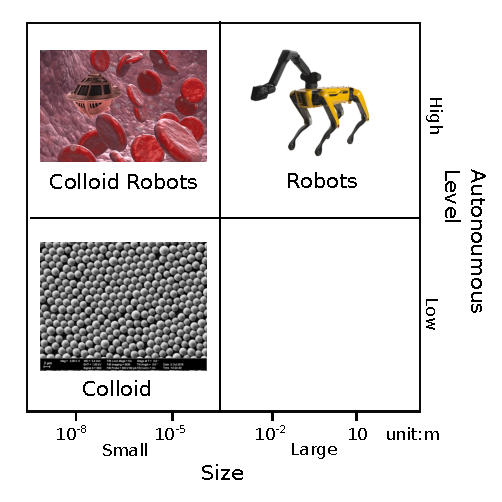
\includegraphics[width=9cm]{figures/1_1.pdf}
\caption{colloidal robots are a combination of the words "colloid" and "robots". colloidal robots are the same size as colloid particles from $\n m$ to$\mu m$ and usually suspend throughout the liquid phase. At the same colloidal robots show dynamics autonomous behaviors such as motion, navigation, and communication, commonly seen in large robotics or living systems}
\label{fig:1.1}
\end{figure}


\section{Essential components for colloidal robots}
Because colloidal robots are still robots, their design shares some of the same basic principles and knowledge from  macroscopic robotic systems.  Traditionally, robots are divided into three essential parts actuators, sensors, and controllers. For example, consider a popular cleaning robot: the Roomba vacuum cleaner (Figure 1.2).  This robot has two actuator systems: one is responsible for locomotion so that the robot can move around your apartment (wheels); the other is responsible for collecting dust and dirt (brush and vacuum).
The sensors for cleaning robots include infrared  sensors and cameras, which provide information about the environment--for example, the position of obstacles. Using such information, the controllers are programmed  to help cleaning robots plan  the actions. For example, if cleaning robots sense a corner, the controllers will let cleaning robots turn around to avoid crashing. One different thing about controllers is that controllers don't necessarily have physical parts. A controller can be a algorithm or a simple math function.  For all the robots, sensor , actuators, and controllers must work together as a feedback loop so robots can work functionally to finish different task: sensors collect information from the environment; based on information from sensors as well as the target of robots,  controllers will make decisions  on how to move actuators; then the actuators will drive robots into a new environment to repeating this feedback loop. This feedback loop composed of actuators, sensors,  and controllers is also the design guidance to build a colloidal robot. However, due to size limitation and different physics regime of colloidal robots, new mechanisms of actuation, sensing and controlling should be developed compared to the conventional approach in the large scale robots.  In the next section, we will address the challenge to build a colloidal robot. 

\begin{figure}
\centering
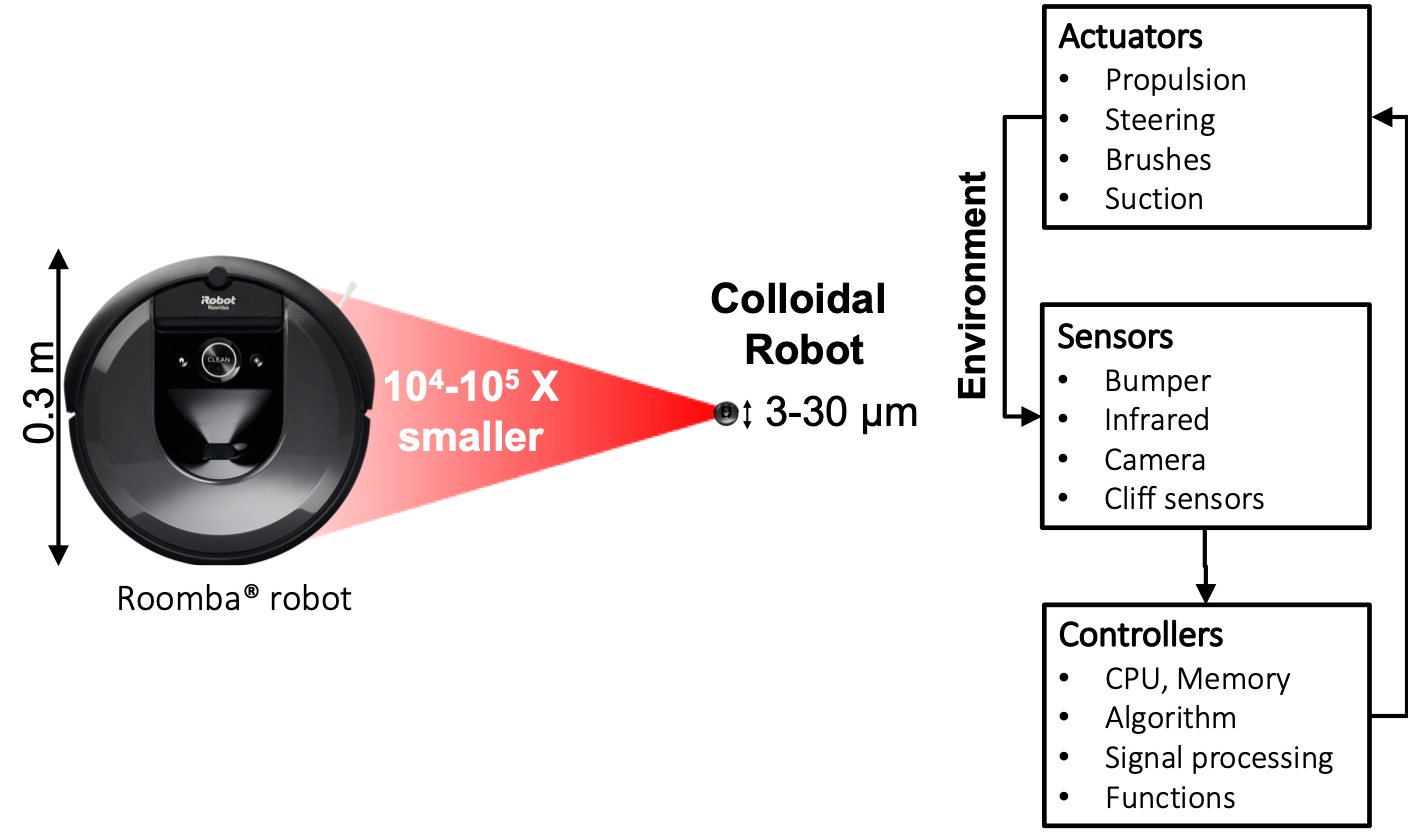
\includegraphics[width=12cm]{figures/1_2.png}
\caption{The essential components and feedback to design a colloidal robot. In the feedback loop, sensors continuously collect information for controllers. Based on  information from sensors and targets of a robot, controllers will make decisions on how to drive the actuators.}
\label{fig:1.2}
\end{figure}

\section{The challenge to  build colloids robots}

\textbf{Size limitation}. In addition to the three basic components (sensors,actuators, and controllers) in the feedback loop, a robot also needs power supplies, manipulators with joints and a body frame, etc. Even for the simplest clean robot, there are around 100 parts inside. It is not possible to integrate all of these complex components in a micron-size particle (a micron size particle on a cleaning robot is just like a human standing on the earth)  if we simply follow the conventional method to build a normal size robot. 

\textbf{Physics limitation}. Physics for a colloid scale particle in the squishy  environment is very different from our normal size world, where everything becomes noisy and sticky. First, in the colloidal scale, Brownian motions largely affect the dynamics of colloidal particles, adding stochastic influence to the robotics. These thermal motions increase the difficulties in controlling the colloidal robot's accuracy and precision. This requires the mechanism to drive colloidal robots to be reliable enough to overcome the background noise. Second, the inertia totally disappears in the small scale as the Reynolds number of the colloidal robot's system approach 0.  The Reynolds number presents the ration of inertia and viscosity represented as
\begin{equation}
    Re=\frac{\rho v l}{\mu}
\end{equation}
where $\rho $ is the density of fluid environment, v is the velocity of particle, l is the size of particle. $\mu$ is the  viscosity of fluid. In the colloid scale, both size and speed of particles are much smaller than 1, leading to the Reynolds number almost 0. The absence of inertia means all of the actuation method in normal size robots based on inertia will no longer work. This interesting  motion restriction in low Reynolds number is called Scallop
theory and was first discussed by Edward Purcell (Professor Prucell was famous for his independent discovery of something else (nuclear magnetic resonance, NMR), which brought him a Nobel prize) \autocite{purcell1977life}. As shown in figure 1.3, Scallop Theorem states that a swimmer which exhibits time-symmetric motion cannot achieve net displacement in a low Reynolds number fluid environment because all the motion is time reversal. There is no difference between closing a scallop and opening a scallop. New actuation methods different large robot systems for colloidal robots must be 

\begin{figure}
\centering
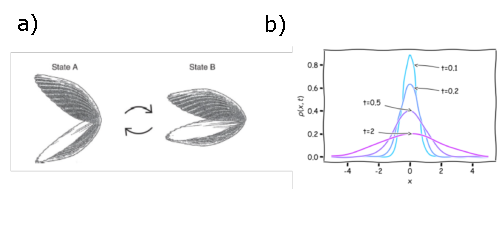
\includegraphics[width=8.5cm]{figures/1_3.pdf}
\caption{Physics challenge for building a colloidal robot (a) Scallop theory. In the colloid scale, the effect of inertia almost disappears, making everything time reversal. (b) Brownian motion. The presence of thermal noise in the colloid scale let the motion of colloidal robots unpredictable.}
\label{fig:1.3}
\end{figure}
To solve the  challenges mentioned above and design the colloidal robots, researchers got inspired from real small living  machines. The dynamic functions of living cells require integration of structures and processes to drive material organization in space and time. For example in the muscle cell,  the coupling of complex structures (kinesin motor protein) and dissipative processes (ATP hydrolysis) can generate mechanical work (see fig 1.4). Thus, a colloidal robot should also have both complex structures and a dissipative process. Thanks to the development of nano/micro scale fabrication in the semiconductor industry, we can now create materials with heterogeneous structure and composition on length scales spanning molecular to macroscopic dimensions with chemical synthesis, lithography, deposition , and etching. These technologies can be directly transplanted to the fabrication process of colloidal robots. In addition to structural and material complexity, the artificial dissipation process (or actuation process) for colloidal robots  can be generated  with chemical reaction, external field (electric, magnetic, acoustic or fluid flow) to generate motion breaking the time reversal constraint. For the past decade, lots of research has been conducted to engineeringly build colloidal robots  or study the fundamentals of colloidal robots. The colloidal robot is now a emerging interdisciplinary field attracting many scientists with different background from math, physics to chemistry, biology and engineering. A state-of-art  review on colloidal robots' research is going to be reviewed in the next section.
\begin{figure}
\centering
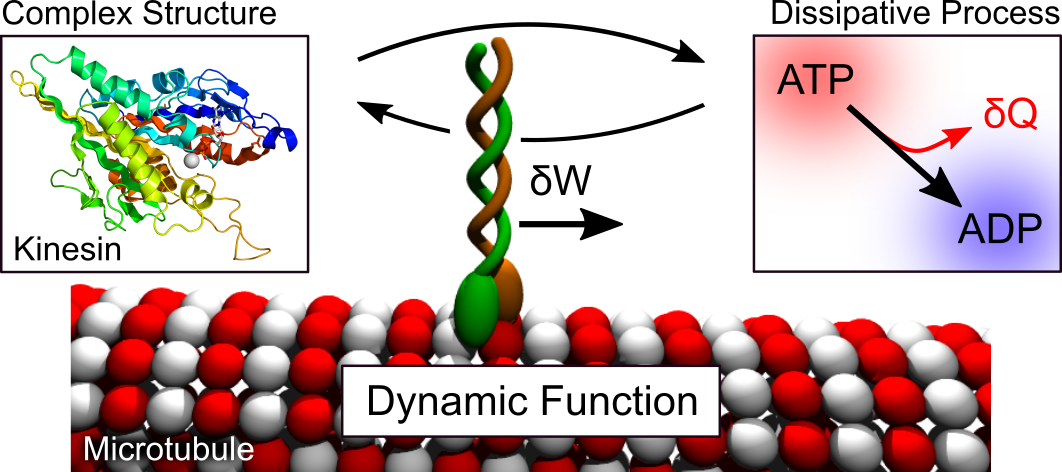
\includegraphics[width=8.5cm]{figures/1_4.png}
\caption{Dynamic functions require the coupling of complex structures and dissipative processes–here, a kinesin motor protein bound to a microtubule  does work powered by ATP hydrolysis}
\label{fig:1.4}
\end{figure}

\section{A state of art review on colloidal robots }
It is not clear which paper first mentioned the similar idea of colloid scale robotics (the original concept of  small scale machines can be tracked to Richard Feynman's famous paper,\textit{There's plenty of room at the bottom}\autocite{feynman1960there}). The current research wave in the past decade on the colloidal robots is triggered by the discovery of self propulsion active colloid particles driven by chemical fuels \autocite{paxton2004catalytic}. In 2004, scientists from Penn State University found that chemical fuel (they use hydrogen peroxide, $H_2O_2$,  in their first paper) can drive  gold-platinum bimetallic nanorods' autonomous motion. The asymmetric different chemical reactions, which happen at the different end of their nanorod,  lead to a net flow fluid near the surface of nanorod. This pioneer research then attracted lots of attention in different research field beyond chemistry such as soft condensed matter physics\autocite{Marchetti2013}, materials science\autocite{han2018engineering}, applied math\autocite{fodor2016far} and engineering \autocite{sitti2015biomedical}. More than tens of thousands of papers related to the autonomous behaviors of colloids have been published since then. However, most of these research papers either experiment or theory only focus on building actuators for colloidal robots. Only a few of them realize some complex tasks with colloidal robots such as navigation. From our knowledge, the higher level's automation is still challenging, and should be the main research direction in the future. In the following content, we are going to give a short state-of-art review on both experiment approach to colloidal robots as well as some basic theories and simulation methods for colloidal robots. In this short review, we have no intention and interest to rephrase and cover all the research papers on colloidal robots like an encyclopedia book. Instead,  I will focus on the main physics, chemistry and engineering ideas behind these papers. 

\subsection{Experiment approach}

\textbf{Fabrication}  High throughput nano/micro scale fabrication technologies in semiconductor manufacturing industry now can make a 3-D structure even smaller than 5 nm \autocite{mokhlesi2010three}. These fancy technologies to make CPU and memory in electronic devices can be transplanted directly to make colloidal robots with almost any desired size, shape and component in cleanroom\autocite{koman2018colloidal}. A typical fabrication process mainly including lithography to make patterns as the main body and frame for colloidal robots , etching to remove unnecessary materials and deposition to introduce new materials. Multi-layer processing can be designed and optimized to make high dimensions and complex structure such as spiral shape\autocite{zhang2009artificial}. After the colloidal robots are fabricated on the wafer, they can be harvested from the silica surface with etching technology or simply physical removal. For the detailed process of fabrication, I would like to refer readers to these three comprehensive reviews\autocite{wong2016synthetic,wang2017emerging, zha2018tubular}. Chemists and material scientists also contributed creative chemical synthesis methods to make colloid scale complex structure with one-pot high-throughput method\autocite{youssef2016shape,gong2017patchy,wang2019active}. One challenge for colloidal robots' fabrication is to   make  colloid scale soft (or shape-shifting) structures with complex components. Liquid crystal, hydrogel gel, droplet, silica polymer and self-assembled nanoparticles are promising candidate materials for micro/nano scale soft structure. \autocite{leong2009tetherless,denkov2015self,zhang2017printing,wei2019molecular}. Another fabrication challenge is to make bio-hybrid colloidal robots which can take advantage of  properties in real living systems. Bio-hybrid colloidal robots require high compatibility  among different materials, where experimental biologists can provide invaluable experience and knowledge\autocite{stanton2016biohybrid,magdanz2013development}.

\textbf{Actuation} Autonomous motion is the most basic characteristic of colloidal robots, making colloidal robots real machines instead of simple colloid particles. colloidal robots can harness energy from the environment and convert energy into mechanical work. Compared to the inertia driven mechanism in normal size robot, the actuation of colloidal robots always experiencing large hydrodynamics resistance force to balance the driving force. The actuation's power source can be divided into two main categories: chemical/biochemical reactions and the external physical fields. Living cells and bacteria use a series of  chemical reaction networks (e.g. ATP hydrolysis) to convert their food source to motions. colloidal robots can also mimic this life-like energy conversion mechanism by implementing the chemical reactions on the surface of colloid particles. The reactions happen between the material of colloidal robots and chemical species in the fluid environment. colloidal robots can work as a catalyst or reactant to trigger the reaction in the fluid environment. For example,  colloidal robots can be made of gold or metal,  which catalysis the hydrogen peroxide in the fluid to water and oxygen. During the fabrication process, these catalysis or reactant material are patterned at different places of colloidal robots to break the symmetry generating chemical species' gradient or reaction product (e.g. bubbles) to actuate colloid particles \autocite{velegol2016origins,shklyaev2016harnessing,parmar2018micro}. Recent reports also showed biochemical reaction (e.g. enzyme) can be options to drive colloidal robot's motions, although the mechanism is still controversial\autocite{zhao2018substrate,somasundar2019positive}.

In addition to  chemical reactions, almost all the external physical field have been used to powering autonomous motion of colloidal robots including electric\autocite{lee2019directed}, magnetic\autocite{zhang2009artificial}, acoustic\autocite{sabrina2018shape}, light\autocite{dai2016programmable}, or thermal field\autocite{lozano2016phototaxis}.  Colloidal robots programmed with physical monopole, dipole or quadrupole will respond to the external physical fields, leading to rotational or transitional motion. For example, colloidal robots can be fabricated with magnetic materials such as nickel and cobalt to a have magnetic dipole moment. Then an external magnetic can generate a torque on the colloid's magnetic moment, manipulating the autonomous motion. Compared to the  chemical reaction actuation method, an external physical field can drive colloidal robots' motion with less fluctuation. \autocite{han2018engineering,ren2018two}. 
The current biggest issue in actuation of colloidal robots is the very low energy efficiency (usually in the order magnitude of $<10^{-5}$ or less). colloidal robots always dissipate large amounts of heat\autocite{wang2013understanding} compared to the real living cells which can perform efficient motion with much less heat dissipation.

\textbf{Coupled actuation}  In addition to a single colloid particle's actuation,  colloidal robots can also be actuated via many actuators' interaction and coupling similar to the multi-cylinder engine in a car. These coupled actuation behaviors can perform some life-like collective functions seen in birds' swarm and fish's flock \autocite{wang2015one,ginot2018aggregation}. Emergent patterns, dynamic clustering, and phase separation have been observed  in different colloidal robot systems. \autocite{buttinoni2013dynamical,ginot2018aggregation,duan2013transition,theurkauff2012dynamic} The interactions among colloidal robots are usually in two forms. One is pure force interaction with each other. For example charged colloidal robots have electrostatics interactions. \autocite{dou2018emergence} The second kind of interaction is indirect influence. One colloidal robot's motion and dynamics  will have an influence on the fluid environment, then  the fluid environment will exert this influence back to other colloidal robots in the same environment. Most of the second type interactions are hydrodynamic or chemical reactions. For example, the hydrodynamics flow induced by one colloidal robots will attract/repel other colloidal robots from it. \autocite{karani2019tuning} Although colloidal robots showing collective behaviors can interact with each other, this kind of communication and interaction is passive and lack of programming. colloidal robots cannot take pre-programmed actions from controllers for some desired tasks when they are exerted on some interactions--most papers studying collective behaviors of colloidal robots only observe the phenomena instead of  programming the dynamics.  As a comparison, in normal size robots research, distributed robotics or  swarms robotics\autocite{wei2010sambot,arvin2014colias} can also show life-like dynamics behaviors, but they are more intelligent. These robots can communicate with the electronic signal instead of pure physics force. They can not only interact with each other, but also perform programmed reactions and different tasks\autocite{rubenstein2012kilobot,rubenstein2014programmable,li2019particle}.

\textbf{Navigation} All the living cells or batteries can sense the information from the environment to navigate themselves for energy, food, or suitable living place called \textit{taxis} behaviors. Autonomous colloidal robots should capable of the same kind of navigation abilities. Not so many experiments approach haven been showed to demonstrate  artificial taxis in colloidal robots compared the large amounts of papers on simply showing autonomous motions. Current approaches mainly belong to two mechanisms: computational vision feedback system and physical force "correction" method. The computational vision feedback system uses a microscope with digital camera to track the location and velocity of colloidal robots online with a computer vision algorithm. Then based on the information of location, speed of colloid particles, and the desired navigation direction, the computer (controllers) will compute the proper external field that should be applied in the next time point. The "tracking-computing-applying new field" feedback loop will continue until colloidal robots reach the destination\autocite{li2017autonomous,han2017sequence} This method has several big defects. The first disadvantage is the size of the whole system. The navigation behaviors have to be coupled with complex external devices (microscope, camera, computer) which is not portable and convenient. Second, this mechanism cannot apply to a large number of colloidal robots with different location and velocity because the external physical field can only satisfy one particle's navigation requirement. The physical force "correction" method can navigate  colloid to transport following  some gradient information mimicking a living taxis behavior. This method uses the local gradient information (e.g.light intensity, chemical species concentration, temperature) or asymmetric geometry to generate torque rotating  the colloidal robot to "correct" its orientation aligning with the gradient. Then the colloidal robot can move along with gradient in the environment showing navigation behaviors \autocite{brosseau2019relating,ten2014gravitaxis,lozano2016phototaxis,baker2019fight} However the physical force correction method  lacks the robotic feedback with controller and sensors. With this mechanism, a colloid particle can only be navigated into one direction, which can't be easily re-programmed for doing other types of navigation tasks in a different environments. All of the problems for the current approach to autonomous navigation mentioned above is due to the lack of sensors and controllers in the colloid scale for colloidal robots





\subsection{Theory and simulation}
Richard Feynman said "What I cannot create, I do not understand." to emphasize the importance of fundamental understanding of science. This is also true for the  research in colloidal robots. To design a colloidal robot of higher automation level, understanding the physics and mathematics behind it is as  important as  experimental attempts. colloidal robots are operated far from the equilibrium state with constant energy and mass flow. Recently years there has been intensively research on non-equilibrium matter, called active matter, in the community of soft matter and statistic physics. Some study is focusing on building a generally high-level theoretical physics framework for active matter with continuum mechanics or statistical mechanism. \autocite{stenhammar2013continuum,solon2015pressure,fodor2016far}. Lots of papers are also trying to use simulation or toy models to discover and design new dynamics behaviors in colloidal robots. \autocite{bechinger2016active,speck2014effective,ten2011brownian}. In this section,  basic physical features and mathematical descriptions are going to be reviewed for colloidal robots.  Deeper and detailed derivation can be referred to our citations.

\textbf{Brownian motion} colloidal robots' motion is influenced by the thermal noise (Brownian motion) in the fluid environment because of their small size. The Brownian motion can be described with Einstein–Smoluchowski Diffusion Equation\autocite{islam2004einstein}. If we take the colloidal robot as  a rigid spherical body, the translation and rotation diffusion coefficients are: 

\begin{equation}
    D_T=\frac{k_B T}{6 \pi \eta R }
\end{equation}
\begin{equation}
    D_R=\frac{k_B T}{6 \pi \eta R^3 }
\end{equation}
where $k_B$ is the Boltzmann constant, $T$ is temperature of the environment, and $\eta$ is the viscosity of fluid, $R$ is the radius of colloidal robots. The diffusion characteristic time is the 
reciprocal of diffusion coefficient, as  $\tau=D^{-1}$. As the size of colloidal robots decrease, the rational diffusion coefficients$D_T$ increase much faster than transnational diffusion coefficients$D_R$. For an actuated colloid with autonomous motion velocity as $v$ in two dimensions, the dynamics can be described as,
\begin{equation}
    \frac{dx}{dt}=v Cos(\theta)+\sqrt{2 D_T}\xi_x, \quad \frac{dy}{dt}=v Sin(\theta)+\sqrt{2 D_T}\xi_y,\quad
    \frac{\theta}{dt}=\sqrt{2 D_R}\xi_\theta
\end{equation}
Where $\xi$ is the independent noise with mean as $0$ and correlation as $\delta(t)$. In chemical engineering, we use the Péclet number to represent the dimensionless ratio between convection  and diffusion. For colloidal robots, the Péclet is 
\begin{equation}
    Pe\propto\frac{v}{\sqrt{D_T D_R}}
\end{equation}
to characterize the influence of Brownian motion on the actuated autonomous motion.

\textbf{Actuated force} As introduced in the previous section, actuation mechanisms are divided into chemical reactions and physical field actuation. For the chemical reactions driven colloidal robots, the phoretic interaction  model describes the system very well. \autocite{golestanian2007,najafi2004simple,golestanian2005propulsion,golestanian2019phoretic} In this model, the reaction rates are considered much faster than the diffusion rate of chemical species, resulting in the following   
quasi-stationary reaction-diffusion equation,
\begin{equation}
    -D\nabla^2 C=0
\end{equation}
where D is the diffusion coefficient of reactant, this is the Laplace equation for concentration in the fluid environment. The boundary condition for this Laplace equation is  colloidal robots' consuming or producing chemical species as,
\begin{equation}
    -D \texbf{n}\cdot \nabla C|_{r=r_s}=\alpha(r_s)
\end{equation}
where $r$ is the distance from the center of colloid, $r_s$ is the radius of colloid, \texbf{n} is the normal vector on the surface of colloid and $\alpha(r_s)$ is the flux rate. The chemical reaction will lead to a net normal flux(denoted as $\alpha(r_s)$ ) on the surface of colloid. The fluid will response to the local gradient change near the colloids and generate a slip velocity as,
\begin{equation}
    v_s=\mu(r_s)(\textbf{I}-\textbf{n}\textbf{n})\cdot \nabla C(r_s)
\end{equation}
$\mu$ is called mobility measuring the response rate of fluid to the concentration gradient. By making $\alpha$ and $\mu$ positive or negative, the asymmetric chemical activity on the surface can lead to autonomous motion.  Also, both repulsion and attraction forces between colloids can be achieved to study collective behaviors of this system. \autocite{michelin2015autophoretic}

For the external physical field actuation, the force exerted on each component colloidal robot following the corresponding law of physics. For example, charged colloidal robots with charge amount $q$ experienced electrostatic force $Eq$ in the electric field $E$; magnetic colloid with dipole $m$ in a magnetic field $B$ can be actuated with torque $m\times B$.
Then we can calculate the total force and torque on the rigid body colloidal robots via doing the surface integration if the force is exerted on the surface.
\begin{equation}
    F=\oint_S f_e \,dS
\end{equation}
\begin{equation}
    T=\oint_S (x-x_c)\times f_e \,dS
\end{equation}
Where $f_e$  is the component of the actuated force and $x_c$ is the center of colloidal robots.

\textbf{Hydrodynamics}  The in-compressible viscous fluids are governed by Navier–Stokes equations without any inertia component as discussed in the previous section,
\begin{equation}
    \eta \nabla^2\textbf{u}-\nabla p=0,\quad \nabla \cdot u=0
\end{equation}
where $\eta$ is the viscosity, p is the pressure from fluid. Although hydrodynamic problems are the most complex ones in modeling colloidal robots because of non-linear terms, it is also the most interesting modeling research part with lost of  nontrivial and unexpected results and patterns. \autocite{Lauga2009,berke2008hydrodynamic,lauga2011life} In the low Reynolds number regime, the hydrodynamic force will balance the external force generated by the actuation mechanism. Stokesian dynamics are used to calculate the  translation and angular velocity of colloidal robots \autocite{Brady1988a,Kim2005}
\begin{equation}
    \left[ \begin{array}{c} F \\ T \end{array} \right] = \begin{bmatrix} A & B \\ B^T & C \end{bmatrix} \left[ \begin{array}{c} v \\ \omega \end{array} \right]
\end{equation}
where \textbf{A}, \textbf{B}, and \textbf{C} are tensors determined only by the shape and orientation of the colloidal robots. The whole big matrix is called resistance tensor, which can be calculated analytically\autocite{Kim2005}  Tensor \textbf{B} is called coupling tensor to couple the transition and rotation together. Resistance tensor is no longer symmetric if boundary exists in the fluid environment.  Stokesian dynamics  can be extended to calculate the hydrodynamics interactions between each other via Faxen's law.
\begin{equation}
    F_{drag}=6 \pi \eta a((1+\frac{a^2}{6}\nabla^2)v_{\infty}(0)-U)
\end{equation}
Where $F$ is the   force exerted by the fluid on the colloid particles, $a$ is the size of colloid, $u$ is the  the translation  velocity of the colloid and $v$ is the disturbance velocity caused by the presence of other colloids in the fluid environment. We would rather direct our readers to James Swan's paper for the full expression of hydrodynamic interaction in the form of Stokesian dynamics. \autocite{swan2011modeling} Basically, the simulation of colloidal robots' dynamics are solving partial differential equations either numerically or analytically with the physical model showed above. In addition to some commercial multiphysics simulation software such as COMSOL\textregistered, there are also some open-access library written in various coding languages  can help to simulate the dynamics of colloidal robots. \autocite{glaser2015strong,anderson2008general,swan2011modeling,singh2019hydrodynamic}

\textbf{Design and optimization} For engineering purposes, colloidal robots should be designed with desired functions\autocite{liebchen2019optimal}. As shown in figure 1.6 the design process should start with constructing and understanding the design parameters space. For example how many physics variables(e.g size, temperature, fluid viscosity, choice of materials) should be added into our design space. And then we  need to reduce the dimension of the design space based on physics and mathematics to make then design problems easier. Dimension reduction is a very essential part of the colloidal robot's design problem. A good dimension reduction will significantly reduce the time searching for the optimized result. Then we build a physical model to link these design parameters and our target functions of colloidal robots together. This physical model should be adequate enough  to capture call the key physics affecting the dynamics of colloidal robots. At the same time, this model should be concise enough to eliminate unnecessary computation work. After the forward modeling is constructed, we can reverse design the parameter of colloidal robots by defining the desired performance functions such as the highest velocity, lowest efficiency. Then the final step is to use an optimization algorithm to find the optimal parameters in the design space for the reverse problems. \autocite{ward1963hierarchical,nocedal2006numerical} Recent research also shows that machine learning technology can assist to design colloidal robots with impressive efficiency\autocite{yang2020micro,yang2020cargo,yang2019deep,tsang2018self}.
\begin{figure}
\centering
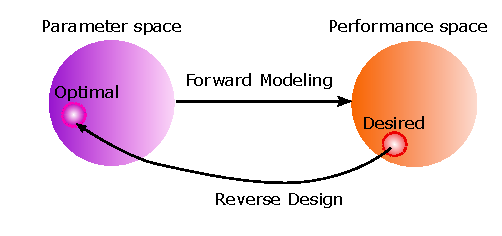
\includegraphics[width=8.5cm]{figures/1_6.pdf}
\caption{The forward modeling connects the design space and performance of colloidal robots together. With the reverse design, the optimal parameters to build a colloidal robot with the desired function can be found.}
\label{fig:1.6}
\end{figure}


%\textbf{Potential Application }


%%%%%%%%%%%%%%%%
% Chapter 2
%%%%%%%%%%%%%%%%

\chapter{Directed motion of metallodielectric particles by contact charge electrophoresis}


%%%%%%%%%%%%%%%%%%%%%%%%%%%%%%
\section{Introduction}

Self-propelled colloidal particles harness energy from their environment to power directed motions relative to their fluid surroundings \cite{Ebbens2015,Li2016,Dey2016}.
Inspired by the locomotion of micro-organisms \cite{Lauga2009}, these artificial swimmers are actively pursued for their potential to navigate complex environments \cite{Takagi2014,Das2015} and deliver cargo to targeted locations\cite{Gao2015,Baylis2015}.
Fluid flows induced by particle motions can also serve to enhance rates of mass transfer to/from the particle surface with emerging applications in water remediation\cite{Soler2013,Li2014} and chemical detection\cite{morales2014micromotor,kagan2009chemical}.
When many self-propelled particles get together, they often interact to form dynamic assemblies\cite{Wang2015} such as swarms\cite{Ibele2009,Nguyen2012}, flocks \cite{Bricard2013}, clusters\cite{JieZhang2016}, and crystals \cite{Palacci2013}.
Synthetic realizations of such active matter\cite{Marchetti2013} provide useful models by which to explore the many forms of self-organization that arise outside of thermodynamic equilibrium.
Importantly, the diverse behaviors of motile particles depend critically on the specific mechanism of self-propulsion and on the associated interactions among the particles.
Expanding the repertoire of colloidal self-propulsion can therefore enable the discovery of new dynamical behaviors as well as the development of future applications.

A wide variety of physicochemical mechanisms have been applied to power the self-propulsion of colloidal particles.
Self-phoretic mechanisms\cite{Golestanian2007} use asymmetries in particle shape and/or composition to create local gradients in the electric potential\cite{Brown2014}, chemical composition\cite{Howse2007}, or temperature\cite{Jiang2010} that drive particle motions via interfacial phoretic effects such as electrophoresis, diffusiophoresis, or thermophoresis, respectively\cite{Anderson1989}.
In a classic example\cite{Paxton2004,Fournier-Bidoz2005}, bimetallic nanorods move autonomously through a homogeneous liquid containing a suitable chemical fuel via reaction-induced  self-electrophoresis\cite{Wang2006,Moran2010}. 
Self-propelled motions of asymmetric particles can also be powered by external fields.
Alternating electric fields drive motions of polarizable particles by induced charge electrophoresis \cite{Squires2006,Gangwal2008,Boymelgreen2014}; alternating magnetic fields power the swimming of flexible magnetic particles by inducing non-reciprocal beating motions \cite{Dreyfus2005}; acoustic fields propel dense metallic particles by directing steady streaming flows\cite{Wang2012,Nadal2014,Ahmed2015}. 
These examples of field-driven particle motion are generally considered forms of self-propulsion, as they allow particles to move freely in multiple directions (typically those perpendicular to the applied field).
The use of external fields to power such motions is attractive for studies of active matter as their magnitude is tunable in space and time.

Here, we describe a type of colloidal self-propulsion in which an electric field drives the autonomous motion of metallodielectric Janus particles\cite{Perro2005,Pawar2008} within an insulating liquid between two plane electrodes (Fig.~\ref{fig:1}a).
Similar configurations have been used to investigate particle motions powered by induced charge electrophoresis within conductive liquids\cite{Boymelgreen2014} and by Quicke rotation within weakly conductive liquids \cite{Bricard2013}.
By contrast, field-driven  motion of conductive particles in insulating liquids is driven by contact charge electrophoresis (CCEP) whereby particles acquire charge on contact with a biased electrode and then move in the field emanating from that electrode \cite{drews2013ratcheted,cartier2014microfluidic,drews2015contact}.
In one well studied example, a conductive sphere immersed in mineral oil oscillates rapidly between two electrodes subject to a constant voltage \cite{drews2015contact}.
Each time the particle contacts an electrode, it acquires charge of opposite polarity and moves back towards the other electrode thereby transporting charge down the applied potential gradient.
Harnessing these motions for useful functions requires strategies by which to rectify particle oscillations.
One approach is to modify the electrodes with asymmetric, ratchet-like features that enable directed transport of conductive particles\cite{drews2013ratcheted} or droplets\cite{Um2016}.
Here, we introduce an alternative strategy that relies on particle asymmetries to achieve similar directed motions.

We show that oscillations of Janus particles between two parallel electrodes are accompanied by steady motions directed perpendicular to the applied field.
Through experiment and theory, we develop and validate a mechanism of self-propulsion whereby the field-induced rotation of the particle upon charge reversal at the electrode surface results in its net displacement during each oscillation cycle.
Repeated displacements in a common direction propel Janus particles at speeds of up to $600~\mu\text{m/s}$ along wide circular arcs within the plane of the electrodes.
Beyond the dynamics of individual particles, we show how particles can both attract or repel one another depending on their separation and on the phases of their respective oscillations.
Together, these results demonstrate how particle symmetry can be used to direct the motions of active colloids powered by CCEP.
The ability to engineer the motions of individual particles and their assemblies will ultimately contribute to the realization of colloidal machines that organize and operate autonomously to perform useful functions \cite{Spellings2015}.

\begin{figure}[p]
\centering
\includegraphics[width=9cm]{2_1.pdf}
\caption{ (a) Schematic illustration of the experimental setup. A metallodieletric Janus particle is immersed in mineral oil between two parallel ITO electrodes (left).  Application of a constant voltage $V$ results in the oscillatory motion of the particle via contact charge electrophoresis (CCEP; right). (b) When imaged from above, the particle moves in and out of focus in time as it oscillates between the electrodes. (c) Over many oscillation cycles, the particle moves steadily away from its conductive hemisphere (top); the steady motion of the particle continues over hundreds of microns (bottom).  See supporting videos 1, 2, and 3.}
\label{fig:1}
\end{figure}
 
 
%%%%%%%%%%%%%%%%%%%%%%%%%%%%%%
\section{Experimental Section}

In a typical experiment, a dilute suspension of Janus particles in mineral oil was sandwiched between two parallel  electrodes separated by a distance $H= 50 - 250~\mu\text{m}$ (Fig.~\ref{fig:1}a). 
We used two types of Janus particles: $8~\mu\text{m}$ silica particles and $4~\mu\text{m}$ fluorescent polystyrene particles, each coated on one hemisphere by a thin layer of gold.
In the absence of an applied field, the particles settled to the surface of the lower electrode where they were imaged from above by an optical microscope.
Application of a constant voltage $V = 200 - 1000~\text{V}$ caused the particles to oscillate rapidly between the electrodes, as evidenced by their periodic appearance and disappearance from the focal plane (Fig.~\ref{fig:1}b). 
Each time a particle came into focus, its position was displaced slightly from that in the previous cycle.
The magnitude and direction of these displacements was relatively constant from one cycle to the next resulting in steady particle motions perpendicular to the applied field.
Using high speed imaging, we quantified the frequency $f$ of particle oscillations as well as the particle position $(x_p,y_p)$ at each oscillation cycle.
For example, at $V = 400~\text{V}$ and $H=200~\mu\text{m}$, a silica Janus particle oscillated between the electrodes at an average frequency of $f = 29~\text{Hz}$ and moved perpendicular to the field at an average speed of $U_{\perp} = 25~\mu\text{m/s}$ (Fig.~\ref{fig:1}c).
Directed particle motion continued over large distances for as long as the voltage was applied.

\subsection{Synthesis of Janus Particles}

Silica Janus particles were prepared by  deposition of gold onto particle monolayers supported on glass slides.
Following Prevo and Velev \cite{prevo2004controlled}, $10~\mu\text{L}$ of a concentrated (30 wt\%) suspension of $8~\mu\text{m}$ silica particles in water was placed between two acid-cleaned microscope slides mounted at an angle on a motorized stage (Harvard Apparatus PHD 2000).
The trapped colloidal solution was dragged at a prescribed speed by the motion of the top slide to achieve well-packed monolayers.
Successive layers of metal (5 nm Ti and 10 nm Au) were then deposited by physical vapor deposition (Cressington 308).

Fluorescent Janus particles were prepared following a procedure adapted from Kopelman et al. \cite{Sinn2011}.
Briefly, sulfonated fluorescent polystyrene particles (ThermoFisher F8858) were washed three times in water by centrifugation and dispersed in methanol at a concentration of 1\% w/v. 
0.5 ml of the particle suspension was deposited onto a 4-inch silicon wafer wafer by spin coating at 2500 rpm for 15 second. 
Successive layers of metal (5 nm Ti, 25 nm Ni, and 20 nm Au) were then deposited by e-beam evaporation (Kurt J Lesker Co. Lab 18). 
The nickel layer was included for a purpose unrelated to the present experiments and is unnecessary here. 
The particles were gently brushed off the wafer using a damp brush.

\subsection{Electrode Configuration}

The electrode setup was comprised of two transparent  indium tin oxide (ITO)-coated glass slides (SIGMA-Aldrich, CAS:50926-11-9, surface resistivity 70-100 $\Omega$/sq) separated from one another by spacers made of glass ($150~\mu\text{m}$ to $250~\mu\text{m}$ thick cover slides) or polydimethylsiloxane (PDMS, $50~\mu\text{m}$ to $100~\mu\text{m}$ thick).
The ITO electrodes were connected to a high-voltage source (Keithley 2410) with a limiting current of $10~\mu\text{A}$ to prevent damage to the system in the event of a short-circuit.
The Janus particles were dispersed in Nylon membrane-filtered mineral oil (SIGMA-Aldrich, CAS:8042-47) at a concentration of $0.01-1~\text{mg/ml}$ and injected into the inter-electrode region.
We note that the charge relaxation time for mineral oil is considerably larger the the timescale of particle oscillations, which is a necessary condition for CCEP \cite{cartier2014microfluidic}. 
The field-induced motion of the Janus particles was captured by a high speed camera (Phantom V310) mounted on an optical microscope (Zeiss Axio Imager A1) operating in bright field mode with 10x and 50x objectives.

\subsection{Particle Tracking}

Movies were captured at frame rates of 1,000 -- 5,000 fps and processed in MATLAB to analyze particle oscillations and reconstruct particle trajectories. 
To determine the oscillation frequency, we first identified a fixed window around a single particle and computed the window-averaged pixel intensity for each frame.
This average intensity oscillated in time as the particle moved into and out of focus, reaching its local minimal value when the particle came into focus at the lower electrode.
For each oscillation cycle $i=1,2,\dots, N$, we identified the time $t_i$ when the particle contacted the lower electrode. 
The mean oscillation frequency was then computed by dividing the number of particle oscillations by the total observation time, $f= N / (\Sigma_i t_i)$.
To reconstruct particle trajectories $(x_i,y_i)$, we considered only those frames when the particle was in focus (i.e., when the average intensity was in local minimum) and determined the location of the particle center using standard algorithms \cite{Track}.
The net displacement for cycle $i$ was computed as $\Delta_i^2 = (x_{i+1} - x_i)^2 + (y_{i+1}-y_i)^2$; the average speed of the particle (parallel to the electrodes) was computed as $U_{\perp} = (\Sigma_i \Delta_i)  /  (\Sigma_i t_i$).

\subsection{Simulation of CCEP Motions}

The model of CCEP dynamics combines classical electrostatics and low Reynolds number hydrodynamics \cite{drews2015contact}. 
The metallic hemisphere of the Janus particle as well as the bounding electrodes are treated as perfect conductors.
To facilitate our numerical analysis, the conductive portion of the particle is modeled as a solid hemisphere with rounded corners (radius $0.1a$) in contrast to the thin hemispherical cap present in experiment.
Additionally, the non-metallic hemisphere and the surrounding fluid are assumed to be dielectrics with a common permittivity $\varepsilon$.
Given the particle charge $q$, orientation $\alpha$, and height $z_p$ above the electrode surface, we solve the Laplace equation numerically to determine the electric potential $\Phi$ and field $\ve{E}=-\nabla \Phi$ throughout the dielectric medium (see Supporting Information for details).
We then integrate the Maxwell stress over the surface of the conductive hemisphere to determine the electric force and torque that drive particle motion.

At low Reynolds numbers (in experiments $Re\leq0.01$), the translational and rotational velocities of the particle are linearly related to the external force and torque by the so-called resistance tensor \cite{Kim2005, Swan2007}.
For a spherical particle near a solid plane boundary, there exist exact analytical expressions \cite{Kim2005} for the components of this tensor, which, when suitably rescaled, depends only on the separation between the sphere and the plane. 
Using these expressions, we compute the particle velocity and integrate numerically to determine the position and orientation of the particle as a function of time.
We assume that the charge $q$ on the particle remains constant until the surface of the metallic hemisphere reaches some critical separation $\delta$ from the plane electrode, at which point charge flows to/from the particle instantaneously to reverse the particle polarity ($q\rightarrow -q$).
Physically, the contact charging process is thought to occur by a type of dielectric breakdown; the resulting charge on the particle is somewhat variable but consistently less than that expected at equilibrium (i.e., when the potential on the particle equals that of the electrode) \cite{drews2015contact}.
After nondimensionalization, the computed particle trajectories depend on just two parameters: the dimensionless charge $q / 4\pi\varepsilon a^2 E$ and the dimensionless separation at contact $\delta / a$.


%%%%%%%%%%%%%%%%%%%%%%%%%%%%%%
\section{Results and Discussion}

Figure \ref{fig:2}a shows the reconstructed trajectories of six different Janus particles under identical conditions over the course of one hundred oscillation cycles based on the experiment results. 
The cumulative displacement of each particle increased roughly linearly with the number of oscillations (Fig.~\ref{fig:2}b) as the particles moved along wide circular arcs of radius $30~\mu\text{m}$ or greater.
These observations are consistent with the spatial homogeneity of the applied field, which suggests that particle motion be invariant to translation and rotation in the $xy$ plane of the electrodes.
Although the majority of particles (ca.~70\% for $V=800~\text{V}$ and $H=200~\mu\text{m}$) exhibited such directed motions, some Janus particles were observed to oscillate between the electrodes with no lateral motion whatsoever.
Additionally, some particles (ca.~20\%) remained ``stuck'' to the electrode surface and did not move at all upon application of the field.

For the particles that moved, the oscillation frequency increased monotonically with increasing voltage as $f \propto V^{2}$ (Fig.~\ref{fig:2}c).
This observation is consistent with previous studies of CCEP motion, which showed that the oscillation frequency scales as $f\sim\varepsilon a V^2 / \eta H^3$, where $\varepsilon$ and $\eta$ are the permittivity and viscosity of the fluid, respectively, and $a$ is the particle radius \cite{drews2015contact}.
By contrast, the lateral displacement of the particle during each oscillation cycle was largely independent of the applied voltage; each oscillation contributed an average displacement of $\Delta = 0.2 a$ (Fig.~\ref{fig:2}d).
Consequently, the lateral velocity of the particle, $U_{\perp}\equiv f\Delta$, also increased as the square of the applied voltage (Fig.~\ref{fig:2}e).
This velocity could be further increased by decreasing the spacing between the electrodes $H$ to increase the magnitude of the applied field (Fig.~\ref{fig:2}f). 
Using spacers of $H=50~\mu\text{m}$, we observed particles velocities up to $U_{\perp}=600~\mu\text{m/s}$ in the direction perpendicular to the applied field.


\begin{figure}[p]
\centering
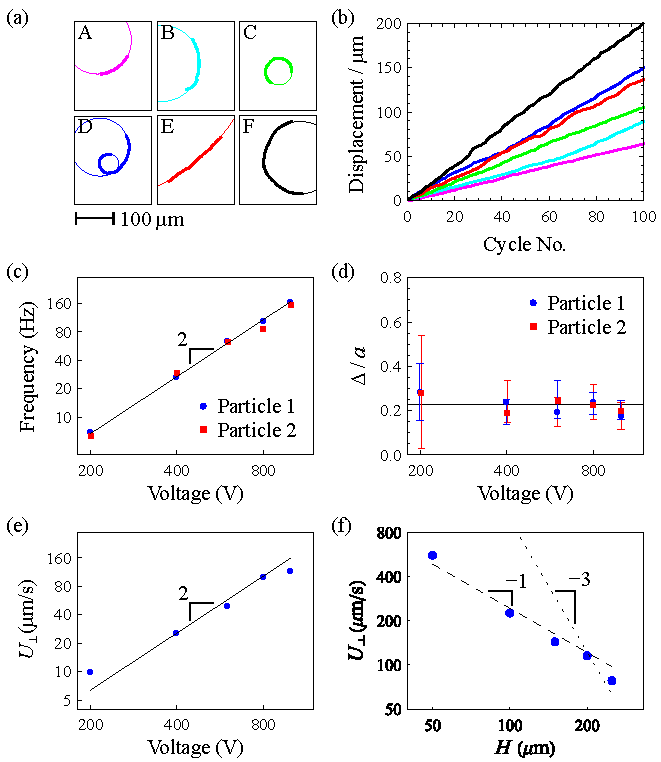
\includegraphics[width=11.2cm]{2_2.pdf}
\caption{(a) Reconstructed particle trajectories of six Janus particles (radius $a = 4~\mu\text{m}$; voltage $V=800~\text{V}$; electrode spacing $H=200~\mu\text{m}$).  Markers denote the particle position at successive oscillations; curves are best circular fits to the data. (b) The cumulative displacement of particles in (a) increases linearly with the number of oscillation cycles. (c) The oscillation frequency of the particle scales quadratically with the voltage.  Markers show data for two independent particles with an electrode spacing $H=200~\mu\text{m}$; the curve is a fit of the form $f\propto V^2$. (d) The lateral particle  displacement $\Delta$ during each oscillation is largely independent of the applied voltage. Markers show the mean displacement; error bars denote one standard deviation above and below the mean. (e) The particle velocity perpendicular to the field scales as the square of the voltage. Markers show data for one particle with an electrode spacing $H=200~\mu\text{m}$; the curve is a fit of the form $U_{\perp}\propto V^2$. (f) Particle velocity increases with decreasing electrode spacing. Each marker represents the velocity of a single particle for an applied voltage $V=800~\text{V}$.}
\label{fig:2}
\end{figure}

To explain these experimental observations, we propose the following propulsion mechanism illustrated in Figure \ref{fig:3}a. 
As it moves across the channel, a charged Janus particle adopts a preferred orientation in which its principal axis is oblique to the applied field and its motion is directed towards the metallic hemisphere.
When it contacts either electrode, the charge on the particle changes sign thereby altering its preferred orientation in the field.
The field-induced rotation of the particle in the vicinity of the electrode surface results in a lateral displacement, which is qualitatively similar to that of a sphere ``rolling'' along the surface.
Successive rotations occur in a common direction towards the non-metallic hemisphere causing a steady lateral motion over the course of many oscillations.
This putative mechanism is supported both by experimental observations of the transient particle orientation and by a mathematical model that describes the electrostatics and hydrodynamics of CCEP motion.

\begin{figure}[p]
\centering
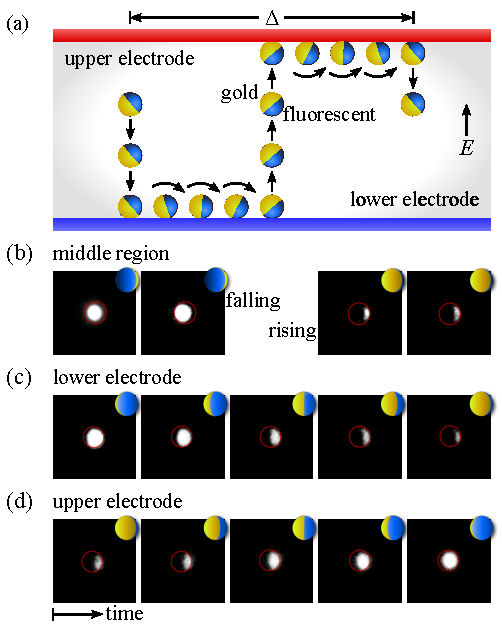
\includegraphics[width=8.5cm]{2_3.pdf}
\caption{(a) Schematic illustration of the propulsion mechanism showing one oscillation cycle.  Rotation of the particle near the electrodes results in a lateral displacement $\Delta$. (b-d) Fluorescent microscopy images highlight the non-metallic hemispheres of fluorescent Janus particles. Images are captured from above; the icons show the particles viewed from above using the color scheme from (a). Particles in the middle region (b) adopt a stable orientation that depends on their direction of travel (falling vs.~rising). Upon contacting the lower (c) or upper (d) electrode, particles rotate in time from one orientation to another. See supporting video 4.}
\label{fig:3}
\end{figure}

We used fluorescent particles to better visualize the orientation of Janus particles moving by CCEP.  
Such particles appeared bright when the metallic hemisphere was directed ``down'' (negative $z$ direction; away from the microscope objective) and dark when the metallic hemisphere was directed ``up'' (positive $z$ direction; towards the objective). 
For intermediate orientations, the fluorescent hemisphere of the particle was partially visible like the bright side of the moon in different phases.
By focusing on planes in the middle of the two electrodes, we observed that particles moving downward appeared bright (gibbous moon) while those moving upward appeared dark (crescent moon) (Fig.~\ref{fig:3}b).
By focusing on the lower electrode, we directly observed the rotation of the particle as it transitioned from the gibbous to crescent configuration (Fig.~\ref{fig:3}c).  
The opposite behavior was observed at the upper electrode where the particle rotated from the crescent to gibbous configuration (Fig.~\ref{fig:3}d).
Importantly, the orientation of the Janus particle in the plane of the electrodes remained relatively constant from one cycle to the next, which allowed the particle to move steadily away from its metallic hemisphere.   

To gain further insights into the propulsion mechanism, we use the equations of classical electrostatics and low-Reynolds number hydrodynamics to describe the dynamical trajectories of Janus particles moving by CCEP.
We first consider the case of a single Janus particle with a net charge $q$ in an unbounded medium subject to a uniform electric field $E$.
We solve for the electric potential within the dielectric and evaluate the electrostatic torque $L(\alpha)$ on the particle as a function of its orientation $\alpha$ relative to the field.
For each charge, there exists one stable orientation for which the electric torque is zero $L(\alpha)=0$ and its derivative is negative $L'(\alpha)<0$ (Fig.~\ref{fig:4}a).
Uncharged Janus particles tend to orient perpendicular to the applied field owing to the increased polarizability of their metallic hemisphere in that orientation ($\alpha=\pi/2$ for $q=0$).
The addition of positive or negative charge, respectively, acts to rotate the particle towards or away from the direction of the field.
When the charge exceeds a critical magnitude, the particle orients perfectly with or against the applied field.
Importantly, this critical charge is similar in magnitude to that acquired by the particle during contact charging (see Fig.~S2). 

\begin{figure}[p]
\centering
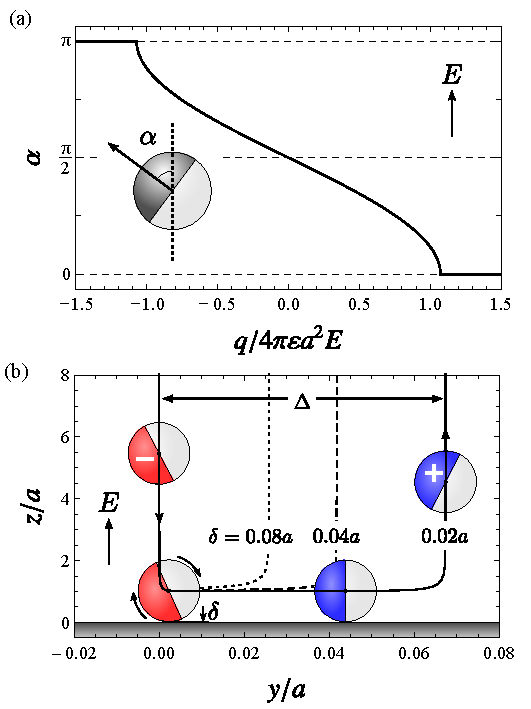
\includegraphics[width=9cm]{2_4.pdf}
\caption{Results of the theoretical model. (a) The stable orientation $\alpha$ of a Janus particle in a uniform electric field depends on the particle's charge $q$ (scaled by $q_s = 4\pi\varepsilon a^2 E$). Uncharged particles align perpendicular to the applied field $E$ ($\alpha=\pi/2$ for $q=0$); highly charged particles align parallel to the field ($\alpha=0,\pi$ for $|q|>1.07 q_s$). (b) Simulated particle ``collisions'' with the lower electrode for a particle charge $q=\pm0.5q_s$. The solid curve shows the trajectory of the particle center; the orientation of the particle at different points along the trajectory is illustrated graphically. The net particle displacement $\Delta$ depends on the surface separation $\delta$ at contact when the particle charge reverses polarity. Note that for clarity the $z$ and $y$ axes use different scales.}
\label{fig:4}
\end{figure}

We now consider the dynamics of a particle ``collision'' with the lower electrode (Fig.~\ref{fig:4}b). 
Initially, the particle is positioned far from the electrode surface ($z_p\gg a$) with some fixed charge $q$. 
We solve for the electrostatic force and torque on the particle and compute the translational and rotational particle velocity in proximity to the surface.
We then integrate these dynamical equations of motion to describe the position and orientation of a single particle as function of time.
Figure \ref{fig:4}b shows three different particle trajectories for different contact separations and a common charge $q = 0.5 q_s$ where $q_s = 4\pi\varepsilon a^2 E$ is a convenient charge scale.
The trajectories are in qualitative agreement with the experimental observations: a particle moves towards the electrode with a preferred orientation, reverses its charge on contact, rotates and translates as it adopts a newly preferred orientation, and ultimately moves away from the surface.
The net lateral displacement $\Delta$ depends on how closely the particle approaches the surface.
For particles that approach more closely to the surface, their rotational motion is more tightly coupled to their lateral translation, and they move farther during each collision.
The displacement also depends on the particle charge in an somewhat surprising way: highly charged particles ($q > q_s$) exhibit little or no displacement (Fig.~S6).
Such particles contact the surface with their axis aligned parallel with field and therefore experience little or no torque upon charge reversal.
Instead, these particles move backward from the surface before ultimately rotating into the new stable orientation; particle rotation far from the surface, however, results in little or no lateral displacement.
This prediction of the model provides a plausible explanation for those particles that oscillate but do not translate perpendicular to the field.

There are some experimental observations that are not captured by the idealized model.
Notably, the model predicts that particles should move along straight lines and not the circular trajectories observed in experiment.
We attribute this discrepancy to defects on the Janus particles that break their axial symmetry.
Imperfections in the particles' metallic hemispheres are known to arise during metal deposition due to shadowing by neighboring particles \cite{Pawar2008}.
Such defects can lead to electric torques about the principle axis of the particle, which are otherwise prohibited by symmetry.
As a result, particles are permitted to change their orientation in the plane of the electrode upon charge reversal.
Understanding these effects requires further study of non-axisymmetric particles of well defined shape.
Interestingly, in some experiments, the curvature of the particle trajectory changed abruptly during its motion (e.g., particle D in Fig.~\ref{fig:2}a). 
This observation may imply that non-axisymmetric particles are capable of multiple ``modes'' of self-propulsion; however, we cannot yet dismiss alternative explanations based on adventurous dust particles.

As noted above, the propulsion velocity is equal to the product of the oscillation frequency and the rotation-induced displacement: $U_{\perp}=f\Delta$.
This expression suggests two basic strategies for maximizing the particle velocity: (i) increase the oscillation frequency, $f\sim\varepsilon a V^2/\eta H^3$, or (ii) increase the lateral displacement upon charge reversal.
The oscillation frequency can be enhanced by increasing the voltage or by decreasing the spacing between the electrodes (Fig.~\ref{fig:2}e,f).
Of course, the electrode spacing cannot be smaller than the particles themselves, and the electric field cannot exceed the dielectric strength of mineral oil (ca.~$5~\text{V/}\mu\text{m}$).
In Figure \ref{fig:2}f, the applied field actually exceeds this threshold value for electrode spacings less than $H=200~\mu\text{m}$; however, device failure was avoided by limiting the current to only $10~\mu\text{A}$.
Under these conditions, the electric field remains roughly constant, and the velocity scales as $U_{\perp}\propto H^{-1}$ (not $U_{\perp}\propto H^{-3}$ as expected for a constant voltage). 
To increase the rotation-induced displacement of the particle on charge reversal, it is necessary to alter the geometry of the particle itself (e.g., the size of the metallic patch). 
Such modifications can be challenging to achieve in practice and their consequences difficult to anticipate. 
Ultimately, the magnitude of the displacement is limited by the size of the particle ($\Delta < a$).

Beyond the motions of individual particles, we observed several interesting  behaviors in systems of two or more interacting particles (Fig.~\ref{fig:5}).
When two particles were separated by a distance less than the electrode spacing ($d<H$), they influenced one another at a distance through electrostatic interactions.
These interactions were either attractive or repulsive depending on the respective phases of the particle oscillations\cite{mersch2011antiphase}.
Like-charged particles oscillating ``in phase'' repelled one another as evidence by an increase in particle separation with time (Fig.~\ref{fig:5}a).
By contrast, oppositely-charged particles oscillating ``out of phase'' moved toward one another in time (Fig.~\ref{fig:5}b).
Due to slight differences in their oscillation frequencies, two particles often transitioned repeatedly between attractive and repulsive regimes.
This particle ``dance'' could end in two different ways: either the particles moved off in different directions to find new partners, or they embraced one another to form a dynamic oscillating chain (a so-called bucket brigade \cite{Pelesko2004a}).
Finally, we observed that interacting particles often moved together in a common direction -- typically, along the line connecting the particle centers (Fig.~\ref{fig:5}c).
Such coordinated motions were considerably faster that the propulsion velocity of individual Janus particles perhaps suggesting an additional strategy for directing CCEP motions.
Importantly, we confirmed that the above effects involving two or more particles were also observed among spherically isotropic (non-Janus) particles.
Understanding the complex dynamics of multiple particles moving by CCEP will require further study beginning with the simplest spherical particles.

\begin{figure}[p]
\centering
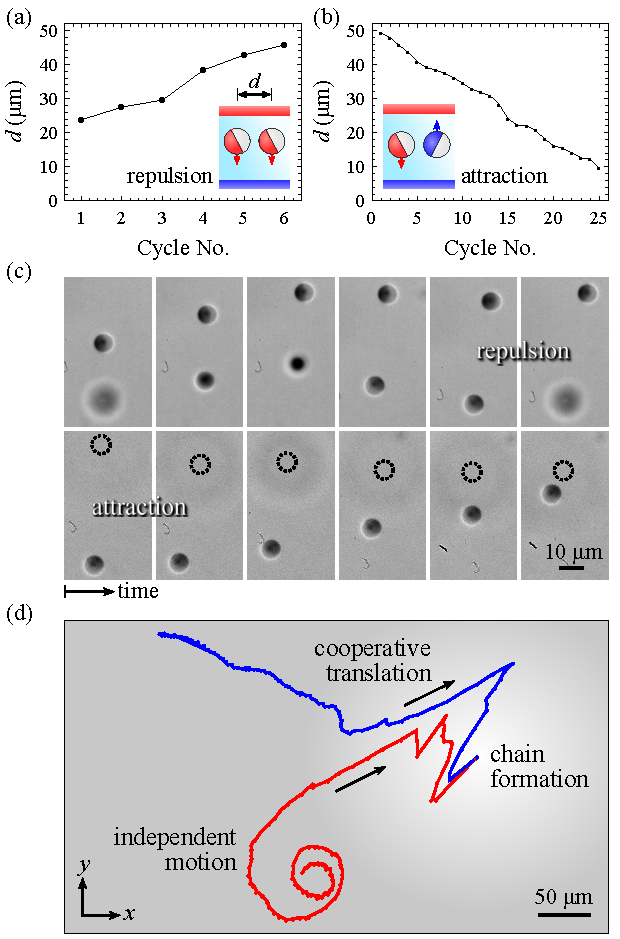
\includegraphics[width=10.5cm]{2_5.pdf}
\caption{(a) The horizontal distance $d$ between two particles oscillating in phase increases during each oscillation cycle. (b) The distance between particles moving out of phase decreases each cycle. (c) Image sequence corresponding to data shown in (a) and (b). (d) Reconstructed trajectories for two interacting particles.  Initially, the particles are moving independently until their separation becomes less than the electrode spacing (here, $H=150~\mu\text{m}$). They then begin to move more quickly in a cooperative manner.  Ultimately, the particles come together to form an oscillating chain. See supporting video 5.}
\label{fig:5}
\end{figure}



%%%%%%%%%%%%%%%%%%%%%%%%%%%%%%
\section{Conclusions}

Contact charge electrophoresis drives the rapid oscillatory motion of conductive microparticles within nonpolar fluids.
Particle asymmetries can be used to rectify such oscillatory motions to achieve directed transport perpendicular to the applied field.
Rectified motions derive from particle rotations near the electrode surface upon contact charge transfer, which lead to repeated displacements in a common direction.
This type of self-propulsion exhibits several characteristics that distinguish it from related systems based on self-phoresis, induced-charge electrophoresis, or Quicke rotation.
Owing to the negligible electric currents through the nonpolar fluid, particle motions are highly efficient and require small energy inputs (ca.~1 nW / particle) \cite{drews2015contact}. 
Rapid particle motions can enhance microscale mixing within nonpolar fluids \cite{cartier2014microfluidic}, which could be harnessed to accelerate catalytic reactions limited by mass transfer.
Long-ranged electrostatic interactions among the particles results in complex collective motions relevant to the study of active matter.
Importantly, the directed CCEP motions of asymmetric particles can in principle be engineered by tuning the particle shape and surface composition.
The rational design of such active components is a critical prerequisite for constructing dynamic colloidal assemblies capable of useful functions -- that is, colloidal machines.


%%%%%%%%%%%%%%%%%%%%%%%%%%%%%%









%%%%%%%%%%%%%%%%
% Chapter 3
%%%%%%%%%%%%%%%%

\chapter{Emergence of traveling waves in linear arrays of electromechanical oscillators}




%%%%%%%%%%%%%%%%%%%%%%%%%%%%%%%%%%%
%%%%%%%%%%%%%%%%%%%%%%%%%%%%%%%%%%%
%%%%%%%%%%%%%%%%%%%%%%%%%%%%%%%%%%%
\section{introduction}
Traveling waves of mechanical actuation provide a versatile strategy for locomotion and transport in both natural and engineered systems across many scales. These rhythmic motor patterns are often orchestrated by systems of coupled oscillators such as beating cilia or firing neurons. Here, we show that similar motions can be realized within linear arrays of conductive particles that oscillate between biased electrodes through cycles of contact charging and electrostatic actuation. The repulsive interactions among the particles along with spatial gradients in their natural frequencies lead to phase locked states characterized by gradients in the oscillation phase. The frequency and wavelength of these traveling waves can be specified independently by varying the applied voltage and the electrode separation. We demonstrate how traveling wave synchronization can enable the directed transport of material cargo. Our results suggest that simple energy inputs can coordinate complex motions with opportunities for soft robotics and colloidal machines.

Traveling waves of mechanical actuation provide a versatile strategy for locomotion and transport in both natural\autocite{Cohen1982, Blake1974, Taylor447} and engineered\autocite{Ijspeert2008, Palagi2016, Park2016, Masuda2016, Yashin2012} systems across many scales. In vertebrates such as the aquatic lamprey \autocite{Cohen1982, Cohen1992}, these and other rhythmic motor patterns are orchestrated by networks of neurons called central pattern generators (CPGs) \autocite{Marder2001}, which are often idealized as systems of coupled oscillators \autocite{Cohen1982, Cohen1992}. The rhythmic output of these oscillators is relayed to actuators (e.g., muscles) to produce complex motions without the need for sensory feedback. Similar control strategies based on CPGs are used to direct  locomotion in macroscopic robots \autocite{Ijspeert2008}. At smaller scales, however, it becomes increasingly challenging to accommodate centralized control systems capable of directing the coordinated actions of multiple actuators. Instead, microorganisms such as ciliated protozoa integrate pattern generation and mechanical actuation within a single material system.  The oscillatory motions of beating cilia couple to one another through hydrodynamic interactions to produce metachronal waves that drive cellular locomotion through viscous surroundings \autocite{Blake1974, Niedermayer2008, Elgeti2013}. This biological example illustrates how the coupled motions of many mechanical oscillators can organize spontaneously and autonomously to perform dynamic functions.

The realization of synthetic systems that mimic such functions requires experimental strategies for powering mechanical oscillators and for coupling their motions to achieve the desired dynamics. One approach relies on coupling reaction-diffusion patterns to the mechanical deformation of responsive gels, for example, to achieve traveling wave motions in excitable media\autocite{Yashin2012,Masuda2016}. Despite fascinating demonstrations of this approach on millimeter length scales, it remains challenging to miniaturize due to the need for faster reactions that compete with diffusion at smaller scales. To achieve scalable mechanisms of pattern formation, the processes that drive oscillations should scale in the same way as those used to couple neighboring oscillators. In this context, electromechanical oscillators based on contact charge electrophoresis (CCEP) \autocite{bishop2018contact, drews2015contact} can provide a useful model on length scales spanning millimeters\autocite{Mersch2011} to microns\autocite{Dou2016} (perhaps even nanometers \autocite{Park2000,Kowalik2016}). 

CCEP refers to the back-and-forth motion of a conductive particle \resp{through an insulating fluid separating} two electrodes subject to a constant voltage. \resp{The particle charges on contact with either electrode and moves down the applied potential gradient, thereby transporting charge between the biased electrodes. This type of electromechanical oscillator is fundamentally distinct from the weakly damped harmonic oscillators of micro-electromechanical systems (MEMS)\autocite{van2011review,Zhang2014}, which rely on resonant excitation by time-varying fields. By contrast, CCEP oscillators are powered by a constant thermodynamic driving force and operate even under conditions of strong damping, which arise at small scales and in viscous environments.  Similar to those of molecular motors\autocite{Kolomeisky2007,Kowalik2016}, CCEP motions can be rectified to perform mechanical work or to transport material cargo\autocite{drews2013ratcheted,Kowalik2016}. Moreover,} the charge acquired by the particle and the forces driving its motion are well described by classical electrostatics, which is invariant to changes in scale. The discovery of new CCEP motions at the macroscale is therefore transferable to emerging applications at the microscale\autocite{bishop2018contact}.

Here, we investigate the collective dynamics of many CCEP oscillators positioned along a linear array between two (nearly) parallel electrodes (Fig.~\ref{fig:1}a). Each oscillator is comprised of a conductive sphere that moves back and forth between the electrodes along a dielectric track.  Oscillatory motions are driven by the repeated charging of the particles on contact with either electrode and their subsequent movement in the applied field. The dynamics of neighboring oscillators are coupled to one another through the electrostatic interactions between the charged particles. We show how this electrostatic coupling mediates the organization of phase-locked states in which all oscillators move with a common frequency. Interestingly, the distribution of oscillator phases at steady state corresponds to traveling waves of particle motion with a characteristic wavelength comparable to the electrode separation. These experimental observations are explained by a Kuramoto-like model\autocite{Acebron2005,Tsimring2005} that accounts for weak repulsive coupling between neighboring phase oscillators and for small systematic variations in their natural frequencies. We demonstrate how traveling wave synchronization can be used to transport material cargo along the length of the oscillator array. More generally, our approach shows how simple energy inputs can power complex patterns of mechanical actuation, which may be useful in powering the motions of soft robots\autocite{rus2015design, acome2018hydraulically} and colloidal machines\autocite{Snezhko2011,Yan2012, Martinez-Pedrero2015, goodrich2017using, Driscoll2017}.

%%%%%%%%%%%%%%%%%%%%%%%%%%%%%%%%%%%
\begin{figure}[p!]
    \centering
    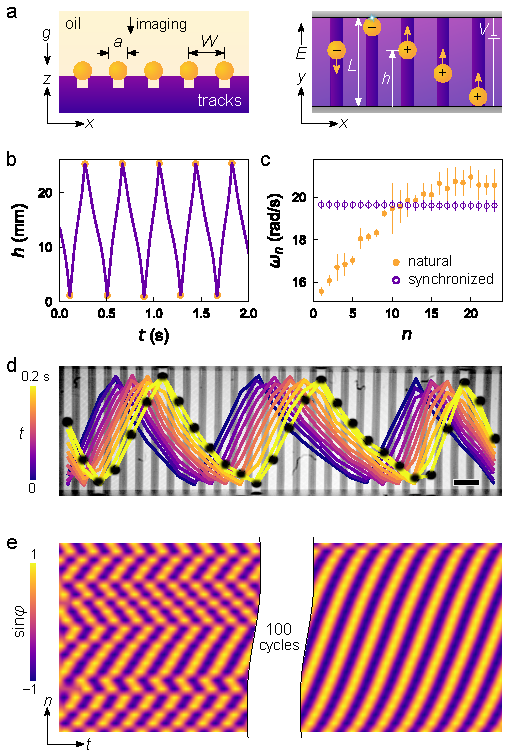
\includegraphics[width=10cm]{3_1.pdf}
    \caption{\textbf{Travelling wave synchronization.} (a) Conductive spheres immersed in mineral oil oscillate along dielectric tracks connecting two plane electrodes subject to a constant voltage $V$. Particles charge on contact with each electrode and move in the electric field $E$. (b) Oscillatory dynamics of a single particle showing its position $h$  as a function of time $t$; yellow markers denote contacts with the electrodes. The applied voltage is $V=19$ kV; the electrode separation is $L=25$ mm. (c) Oscillation frequency $\omega_n$ as a function of the position $n$ along the array. The natural frequency of each oscillator varies with position (solid markers); all oscillators move with a common frequency in the synchronized state (open markers). Error bars represent the standard deviation in the instantaneous frequency, $2\pi/(t_{k+1}-t_k)$, over 100 cycles. (d) Image of the experiment showing particle positions at successive times; scale bar is 3 mm. (e) Space-time plot of the oscillator phase $\varphi$ showing the emergence of traveling wave synchronization for the $N=23$ oscillators in (c) starting from a random initial configuration.  Here, the track period is $W=3$ mm; other parameters are listed in (b).}
    \label{fig:1}
\end{figure}
%%%%%%%%%%%%%%%%%%%%%%%%%%%%%%%%%%%


%%%%%%%%%%%%%%%%%%%%%%%%%%%%%%%%%%%
%%%%%%%%%%%%%%%%%%%%%%%%%%%%%%%%%%%
%%%%%%%%%%%%%%%%%%%%%%%%%%%%%%%%%%%
\section{Results}

\subsection{Experiment}

Copper spheres ($a = 1$ mm in radius) immersed in mineral oil were positioned within an array of dielectric tracks connecting two plane electrodes separated by a distance $L$ (Fig.~\ref{fig:1}a). The tracks were spaced evenly with a period $W=3a$ and aligned perpendicular to the electrode surfaces and to the direction of gravity. Each track contained a single particle, which was free to move back and forth between the two electrodes. Application of a constant voltage (typically, $V=10$ kV) caused the particles to oscillate continuously between the electrodes via contact charge electrophoresis (CCEP) \autocite{bishop2018contact, drews2015contact}. The conductive particles acquired an electrostatic charge on contact with the biased electrodes and moved under the influence of the applied field. This periodic cycle of contact charging and electrostatic actuation continued for as long the voltage was applied.

% Dynamics of individual particles

%\noindent
%\textbf{Dynamics of electromechanical actuator arrays}
Figure \ref{fig:1}b shows the reconstructed trajectory of a single sphere oscillating between the two electrodes. Each time the particle contacts an electrode, its charge changes sign and the particle reverses direction under the influence of the field. To facilitate the analysis of multiple particles over many oscillation cycles, we record the times at which each particle contacts one of the electrodes.  From this data, we approximate the phase of each oscillator by interpolating between successive contacts as $\varphi(t) = 2\pi (t-t_k)/ (t_{k+1}-t_{k})$ where $t_k$ denotes the time of the $k^{th}$ contact and $t_k \leq t < t_{k+1}$. By definition, the oscillator phase increases at a constant rate equal to the natural frequency, $\mathrm{d}\varphi/\mathrm{d}t = \omega$, which is approximated by averaging over many oscillation cycles as $\omega = \langle 2\pi/(t_{k+1}-t_{k}) \rangle_k$. Repeating this analysis for each particle in isolation (i.e., one track at a time), we observed small systematic variations in the natural frequency $\omega_n$ with respect to the oscillator position $n$ along the array (Fig.~\ref{fig:1}c, solid markers). The spatial gradients in the oscillator frequency were caused by small deviations in the electrode alignment,  which was controlled only to within ca.~1$^\circ$ of parallel. Particles oscillated faster where the electrodes were closer together due to an increase in field strength at those locations.
        
% Dynamics of particle arrays
Despite variations in their natural frequencies, linear arrays of $N$ particle oscillators moving simultaneously evolved in time to a phase-locked state, in which each particle moved with a common frequency (Fig.~\ref{fig:1}c). Interestingly, the synchronized particles did not move in phase with one another but rather organized to form a single traveling wave, which remained stable for hundreds of oscillation cycles (Fig.~\ref{fig:1}d; Supplementary Movie 1). Space-time plots of the oscillator phase $\varphi_n(t)$ show how this wave-like pattern emerged from a disordered initial configuration (Fig.~\ref{fig:1}e; see also Supplementary Fig.~1 and Supplementary Movie 2). The direction of wave propagation was related to the spatial gradient in the oscillators' natural frequencies: waves traveled from slower to faster oscillators. Notably, the travelling wave patterns were robust to disturbances and recovered when disrupted by external perturbations (Supplementary Movie 3).

%%%%%%%%%%%%%%%%%%%%%%%%%%%%%%%%%%%
%%%%%%%%%%%%%%%%%%%%%%%%%%%%%%%%%%%
%%%%%%%%%%%%%%%%%%%%%%%%%%%%%%%%%%%

% The role of particle number $N$ 
The stability of the synchronized state and the distribution of oscillator phases therein depended on the number of oscillators $N$ in the array. For $N=2$ oscillators, the particles moved in antiphase as reported previously \autocite{Mersch2011} (Fig.~\ref{fig:2}a). Such antiphase synchronization suggests that neighboring oscillators are coupled together by repulsive interactions such as the Coulombic forces between like-charged particles. As the number of particles was increased, the average phase difference between successive oscillators decreased giving rise to stable traveling waves with wavelengths spanning many oscillators (Fig.~\ref{fig:2}b; see also Supplementary Fig.~2 and Supplementary Movie 4). Beyond some critical number of oscillators $N^*$, the synchronized state became unstable (Fig.~\ref{fig:2}c). Above this threshold, traveling waves were observed to grow and break near the center of the array in a periodic fashion (Supplementary Movie 5). Such breaking events are characterized by dislocation-like defects in the space-time plots for the oscillator phases (Fig.~\ref{fig:2}c). The breaking frequency increased as the number of oscillators was increased beyond the stability threshold $N^*$ (Supplementary Fig.~3). For $N\gg N^*$, wave breaking was no longer periodic but rather occurred at irregular intervals and at different locations (Supplementary Fig.~4 and Supplementary Movie 5).
    
%%%%%%%%%%%%%%%%%%%%%%%%%%%%%%%%%%%
\begin{figure}[p!]
    \centering
    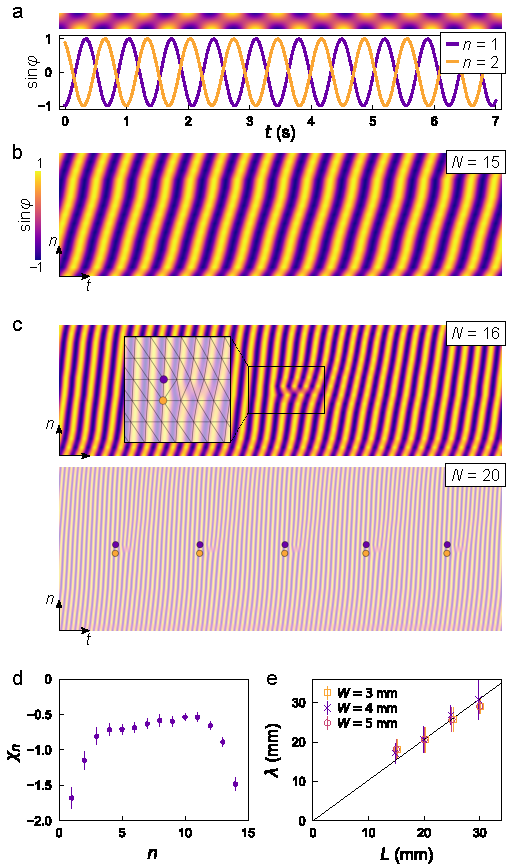
\includegraphics[width=10cm]{3_2.pdf}
    \caption{\textbf{Characterization of travelling waves.} (a) $N=2$ oscillators moving in antiphase. The plot shows the sine of the oscillator phases (bottom); the space-time image shows the same data in a different way (top). (b) Space-time plot for $N=N^*=15$ oscillators showing 20 oscillation cycles. (c) Space-time plots for $N>N^*$ showing defects that occur at regular time intervals. The markers show points in the space-time lattice with five-fold (purple) and seven-fold (yellow) coordination. (d) Time-averaged phase difference $\chi_n$ as a function of position $n$ for $N=N^*$ oscillators. Data for (a-d) were collected with $L=25$ mm, $W=3$ mm, and $V=18$ kV.  (e) Characteristic wavelength $\lambda$ as a function of the electrode separation $L$ for $N=N^*$ and different oscillator spacings $W$. Error bars represent the standard deviation from five independent experiments.}
    \label{fig:2}
\end{figure}
%%%%%%%%%%%%%%%%%%%%%%%%%%%%%%%%%%%

% Characteristic wavelength for $N=N^*$ (Fig.~\ref{fig:3})
To better understand the synchronized state, we quantified the distribution of oscillator phases for $N = N^*$ as a function of the electrode separation $L$ and the oscillator spacing $W$. For each electrode configuration, we started with $N>N^*$ oscillators and removed one particle at a time from the end of the array until reaching a stable synchronized state, at which the phase difference between neighboring oscillators was constant in time. Figure \ref{fig:2}d shows the time-averaged phase difference $\chi^{\s}_n = \langle \varphi_{n+1}(t) - \varphi_n(t) \rangle_t$ at the stationary state for a typical experiment. The phase difference was smallest (in magnitude) near the center of the array and largest near the edges. For each such state, we defined a characteristic wavelength in terms of the average phase difference as $\lambda = 2\pi W / \langle \chi_n^{\s} \rangle_n$. This wavelength increased linearly with the electrode spacing $L$ but was independent of the oscillator spacing $W$ over the range explored (Fig.~\ref{fig:2}e).

%%%%%%%%%%%%%%%%%%%%%%%%%%%%%%%%%%%%%%%
\subsection{Minimal Model of Traveling Wave Synchronization}

The experimental observations are reproduced by a Kuramoto-like model \autocite{Acebron2005} that accounts for the local repulsive coupling between neighboring oscillators and the systematic variations in their natural frequencies.  In the model, we adopt the following simplified description of CCEP dynamics\autocite{Kowalik2016}. \resp{On contact with either electrode, a conductive sphere acquires a charge $q = \pm \tfrac{2}{3}\pi^3\varepsilon a^2 E$, where $E$ is the electric field at the electrode surface, and $\varepsilon$ is the permittivity of the surrounding dielectric.  This expression---first derived by Maxwell\autocite{Maxwell1873}---assumes that charge flows to/from the particle until its potential equals to that of the contacting electrode\autocite{drews2014charge}. The electrostatic force on the particle is approximated as $F = q E$, which drives motion with velocity $U=F/\gamma$, where $\gamma$ is a constant friction coefficient. Figure \ref{fig:4}a shows how the charge $q$ and position $h$ of a single oscillator depend on its phase $\varphi=\omega_{\ro} t$, where $\omega_{\ro} = \pi q_{\ro} E_{\ro}/\gamma L$ is the natural frequency defined in terms of the applied field $E_{\ro}=V/L$ and the Maxwell charge $q_{\ro}=\tfrac{2}{3}\pi^3\varepsilon a^2 E_{\ro}$. By comparing the measured frequency in Fig.~\ref{fig:1}c to the prediction of the model, the friction coefficient can be estimated to be $\gamma=1.8\times10^{-3}$ N s m$^{-1}$, which ca.~4 times larger than the Stokes drag, $\gamma_{\text{s}}=6\pi\eta a$. The increased drag is attributed to the solid boundaries formed by the patterned tracks and the planar electrodes (Supplementary Fig.~5)\autocite{Goldman1967a}.}

% Interactions 
\resp{The presence of neighboring oscillators influences both the charge that a particle acquires and the speed at which it moves.  To describe these interactions, we decompose the electric field as $E=E_{\ro}+E'$, where $E_{\ro}$ is the applied field and $E'$ is a disturbance field due to neighboring particles, which are approximated as point charges (see Methods). In the limit of weak interactions (i.e., when $E'\ll E_{\ro}$), the moving particles are well approximated as phase oscillators with weak repulsive coupling between nearest neighbors.} The phase of the $n^{\text{th}}$ oscillator evolves in time as
\begin{equation}
    \frac{\partial \varphi_n}{\partial t} = \omega_n + f(\varphi_n - \varphi_{n-1}) + f(\varphi_n - \varphi_{n+1}), \label{eq:phase}
\end{equation}
where $\omega_n$ is the natural frequency, and the function $f(~)$ describes the phase-averaged interactions between neighboring oscillators as a function of their phase difference $\chi_n=\varphi_{n+1}-\varphi_n$. The boundaries of the array are open such that oscillators at the edges ($n=1,N$) interact with only one neighbor \autocite{Ottino-Loffler2016}. We assume a uniform gradient in the natural frequency:  $\omega_n = \omega_{\ro} +  \Delta \left[n-\tfrac{1}{2}(N+1)\right]$ for $n=1\dots N$, where $\omega_{\ro}$ is the mean oscillator frequency, and $\Delta$ is the frequency difference between successive oscillators due to a small angle $\theta$ between the electrodes ($\Delta/\omega_{\ro} \approx 3(W/L)\theta  \ll 1$).  Interestingly, this model was investigated previously as a possible explanation for traveling wave oscillations in the central pattern generator of the aquatic lamprey \autocite{Cohen1982}. 

%%%%%%%%%%%%%%%%%%%%%%%%%%%%%%%%%%%
\begin{figure}[p!]
    \centering
    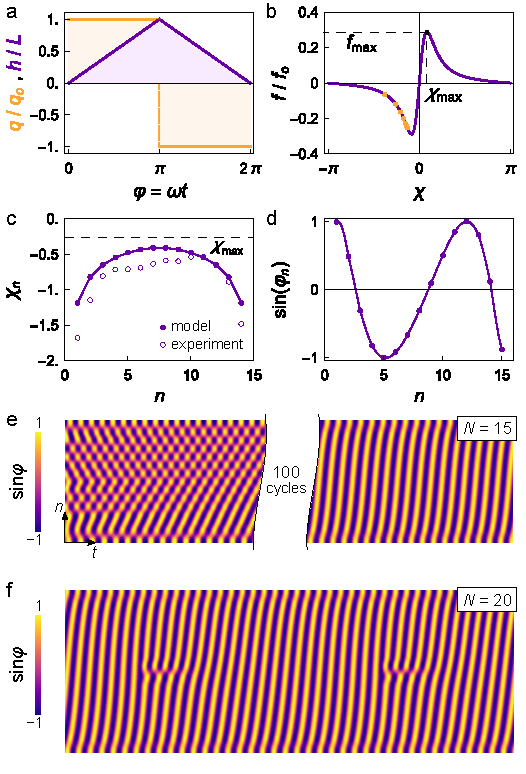
\includegraphics[width=10cm]{3_3.pdf}
    \caption{\textbf{Minimal model of traveling wave synchronization.} (a) Charge $q$ and position $h$ of a idealized oscillator as a function of it phase $\varphi$. \resp{(b) Phase-averaged electrostatic interaction between two weakly-coupled oscillators as a function of their phase difference $\chi$. The interaction is scaled by $f_{\ro} = q_{\ro}^2/\varepsilon W^2 L \gamma$; the oscillator spacing is $W=0.12 L$. (c) Stable stationary solution for the phase difference $\chi_n$ of $N=15$ oscillators. Experimental data for the same conditions is reproduced for comparison. The predicted phase differences are plotted also in (b) to show their relationship with the interaction function $f(~)$. (d) Sine of the oscillator phase $\varphi_n$ showing the wave-like pattern.  (e) Dynamics of the $N=15$ oscillators starting from random initial conditions. (f) Oscillator dynamics for $N=20$ showing the periodic breaking of the traveling waves. In (c)--(e) the critical oscillator number is chosen to be $N^*=15.5$ as in experiment, which implies a frequency gradient $\Delta=0.0096 f_{\ro}$. The natural frequency is $\omega_{\ro}=\tfrac{3}{2\pi^2}(W/a)^2f_{\ro}=1.4 f_{\ro}$ where $W/a=3$ as in experiment; the ratio $\Delta/\omega_{\ro}=0.0070$ implies an electrode angle of $\theta=1.1^{\circ}$.}}
    \label{fig:4}
\end{figure}
%%%%%%%%%%%%%%%%%%%%%%%%%%%%%%%%%%%

% Description of the electrostatic interactions
In the present context, the primary interaction between neighboring oscillators is electrostatic in origin; other interactions are neglected. In particular, the neglect of hydrodynamic interactions was supported by experiments in which neighboring particles were separated by solid walls without altering their collective dynamics (Supplementary Fig.~6).  Approximating the particles as point charges, we compute the electrostatic interaction averaged over one oscillation cycle for a constant phase difference $\chi$ (see Methods). These repulsive interactions are described by an odd function characterized by the location $\chi_{\max}$ and height $f_{\max}$ of its maximum  (Fig.~\ref{fig:4}b).  For large electrode separations ($L\gg W$), these quantities are well approximated as $f_{\max}\approx \tfrac{1}{2\sqrt{3}} (q_{\ro}^2/\varepsilon W^2 L \gamma)$ and $\chi_{\max}\approx\tfrac{\pi}{\sqrt{2}} (W/L)$. \resp{Our assumption of weak coupling implies that the phase velocity due to interactions is small compared to the natural frequency---that is, $f_{\max}\ll\omega_{\ro}$ or, equivalently, $a/W\ll0.72$. Additional simulations incorporating the full amplitude dynamics provide further support for the phase oscillator approximation under the experimental conditions of $a/W=0.33$ (Supplementary Note 1 and Supplementary Fig.~7).}

% Stationary states of the minimal model
The competition between the repulsive interactions and the frequency gradient leads to stable stationary solutions described by $f(\chi_n) = -\frac{1}{2}\Delta n(N-n)$ (see Methods). This solution exists provided that the number of oscillators is below some critical value $N^* = \sqrt{8 f_{\max}/\lvert\Delta\rvert}$. Figure \ref{fig:4}c,d,e shows the stable solution in terms of the phase difference and the sine of the phase for $N=15$ oscillators---just below the chosen critical value of $N^*=15.5$. The addition of more particles ($N>N^*$) causes the waves to break periodically in the center of the array (Fig.~\ref{fig:4}f). Physically, faster oscillators pile up behind the slower ones and are prevented from passing by the local repulsive interactions.  In this way, the frequency gradient acts to compress the oscillator phases together to create longer waves that travel always from slower to faster oscillators. When compression by the frequency gradient exceeds the repulsive barriers between neighboring oscillators, global synchronization is lost and the waves break. 

At the critical oscillator number ($N = N^*$), repulsive interactions are at their maximum ($\chi^{\s}_n \sim \chi_{\max}$), and the characteristic wavelength scales linearly with the electrode separation in agreement with experimental observations (Fig.~\ref{fig:2}e)---that is, $\lambda\sim2\pi W/ \chi_{\max} \sim L$ for $W\ll L$.  Moreover, the critical oscillator number observed in experiment implies a certain angle between the electrodes, which can be estimated from the model as $\theta = \tfrac{1}{3}(L\Delta /W \omega_{\ro} ) = \tfrac{8 \pi ^2}{9 \sqrt{3}} (a^2 L/W^3 {N^*}^2)$. For the conditions of Figure \ref{fig:2}, this angle is predicted to be $\theta = 1.1^\circ$, which agrees well with that measured from the experimental images (Fig.~\ref{fig:1}b).  Smaller angles allow for stable waves containing more particles. 

The average phase within the wave evolves in time at a constant rate equal to the average frequency $\omega_{\ro}$, which is specified independently of the wavelength. In experiment, the oscillator frequency could be altered by changing the applied voltage; however, the range of accessible frequencies was limited by dielectric breakdown at higher voltages and by particle sticking at lower voltages\autocite{drews2015contact}. Notably, the frequency of the phase locked state was slightly faster than the average natural frequency (Fig.~\ref{fig:1}d). Dipolar interactions among the particles (neglected here) break the odd symmetry of the interaction function thereby altering the frequency of the synchronized state.


%%%%%%%%%%%%%%%%%%%%%%%%%%%%%%%%%%%
%%%%%%%%%%%%%%%%%%%%%%%%%%%%%%%%%%%
%%%%%%%%%%%%%%%%%%%%%%%%%%%%%%%%%%%
\section{Discussion}

We have shown how arrays of electromechanical oscillators can organize spontaneously to form synchronized traveling waves of particle motion powered by a constant input voltage.  The direction of wave propagation is determined by small gradients in the natural frequencies of the oscillators and can be controlled by introducing a small angle between the otherwise parallel electrodes.  The characteristic wavelength is approximately equal to the electrode separation $L$ and corresponds to the largest possible wave that can be stabilized by repulsive interactions among the charged particles.  The traveling wave motions are robust to perturbations and can be harnessed to direct the transport of material cargo.  In particular, Figure \ref{fig:5}a shows how traveling waves can direct the motion of gas bubbles floating at the interface just above the oscillating particles (see also Supplementary Movie 6).  Bubbles are transported in the direction of wave propagation at speeds comparable to the wave velocity (Fig.~\ref{fig:5}b). In contrast to previous strategies for rectifying CCEP motions based on ratcheted channels\autocite{drews2013ratcheted} or asymmetric particles\autocite{Dou2016}, the present approach relies on the self-organization of multiple particles working in concert. 

%%%%%%%%%%%%%%%%%%%%%%%%%%%%%%%%%%%
\begin{figure}[h]
    \centering
    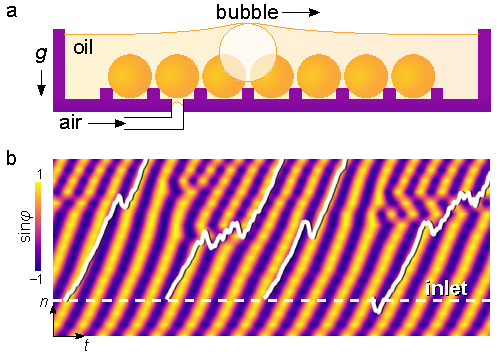
\includegraphics[width=10cm]{3_4.pdf}
    \caption{
    \textbf{Transport of air bubbles via travelling waves.} (a) Schematic illustration of the experimental set-up from the side. (b) Trajectories of four bubbles (white) superimposed over the space-time plot of the oscillator phase. See also Supplementary Movie 6.}
    \label{fig:5}
\end{figure}
%%%%%%%%%%%%%%%%%%%%%%%%%%%%%%%%%%%

\resp{Beyond this initial demonstration, traveling wave synchronization of CCEP oscillators may be useful for peristaltic pumping within microfluidic systems. Unlike standard pressure pumps, those based on traveling wave motions allow for recirculating flows\autocite{mi5020289} and would complement existing  applications of CCEP in microfluidic cargo transport\autocite{drews2013ratcheted,cartier2017electric}, separations\autocite{drews2013ratcheted}, and fluid mixing\autocite{cartier2014microfluidic}. These CCEP-powered unit operations rely on constant voltages at low input power, which makes them attractive for use in portable, battery-powered microfluidic devices\autocite{bishop2018contact}.  One important limitation of these oscillators is their reliance on the dielectric environment provided by non-polar fluids; CCEP motions cannot be sustained in even weakly conductive liquids such as deionized water\autocite{cartier2014microfluidic}. However, recent advances in soft robotics suggest one strategy for circumventing this limitation by encapsulating non-polar liquids in stretchable, impermeable compartments\autocite{acome2018hydraulically}. These soft composite materials can be deformed by applying voltages to stretchable electrodes patterned on their surfaces.  By incorporating arrays of CCEP oscillators within such dielectric compartments, it should be possible to create self-organized motions that drive transient deformations and thereby locomotion of soft robotic materials. } 

%%%%%%%%%%%%%%%%%%%%%%%%%%%%%%%%%%%
%%%%%%%%%%%%%%%%%%%%%%%%%%%%%%%%%%%
\section{Methods}

%%%%%%%%%%%%%%%%%%%%%%%%%%%%%%%%%%%
\paragraph{Experiment Set-up.} 
Periodic arrays of dielectric tracks were 3D printed in acrylonitrile butadiene styrene (ABS) with a period of $W=3-5$ mm. The array was sandwiched between two copper plates separated by a distance $L=10-30$ mm (McMaster-Carr 3350K201) and immersed in mineral oil (Sigma Aldrich CAS No.~8042-47-5). The tracks were aligned perpendicular to the electrode surfaces and to the direction of gravity. Each track contained a single copper sphere (McMaster-Carr No.~64715K16, radius $a=1$ mm), which rolled freely between the two electrodes (Fig.~\ref{fig:1}a). Prior to use, the system was heated in a 60$^\text{o}$C oven for several hours to remove any moisture. The copper electrodes were connected to a amplifier (Trek 20/20C) with an output voltage $V=0-20$ kV.  The particles were illuminated from below by a light emitting diode (LED) and their motions captured by a high-speed camera (Phantom V310).  During each experiment, the electrodes were energized to a specified voltage and the resulting particle motions captured. The voltage was switched off for at least one minute between successive experiments to allow for the dissipation of any space charge accumulated on the surfaces of the tracks and/or the electrodes.  Particle location data were extracted using standard image tracking routines in MATLAB.


%%%%%%%%%%%%%%%%%%%%%%%%%%%%%%%%%%%
\paragraph{Bubble Transport.} 
Bubbles were generated within the oscillator array by a continuous flow of air supplied by a syringe pump at a rate of 0.2 ml min$^{-1}$. The air was delivered through a tube that connected to a hole in the base of one of the tracks (Fig.~\ref{fig:5}a).  The bubbles (ca.~4 mm in diameter) were transported down the length of the array by the coordinated motions of $N=17$ particles of radius $a=1.5$ mm (Supplementary Movie 6).  In these experiments, the applied voltage was $V=18$ kV, the electrode separation was $L=20$ mm, and the height of the mineral oil above the base of the track was 4 mm.  Bubbles were always transported in the direction of wave propagation, which was controlled by introducing a finite angle between the two electrodes.  Control experiments with no applied voltage showed no bubble motion in either direction.


%%%%%%%%%%%%%%%%%%%%%%%%%%%%%
\paragraph{Electrostatic Interactions.}
We first consider a single point charge $q$ positioned at a height $z=h$ between two grounded planes at $z=0$ and $z=L$.  The resulting electrostatic potential at point $\ve{x}$ is 
\begin{equation}
    \phi(\ve{x}) = \frac{q}{\pi L \varepsilon} \sum_{m=1}^{\infty} \sin\left(\frac{m\pi h}{L}\right)  \sin\left(\frac{m\pi z}{L}\right) K_0\left(\frac{m \pi r}{L}\right),\label{eq:point}
\end{equation}
where $r=\sqrt{x^2 + y^2}$ is the radial distance from the charge, and $K_0(~)$ is the zeroth order modified Bessel function of the second kind. For large arguments, the Bessel function decays exponentially as $K_0(s)\rightarrow e^{-s}\sqrt{\pi/2 s} $; the infinite series can be truncated for some $m\gg L/\pi r$ to obtain an accurate approximation.  The corresponding electric field in the $z$-direction is given by $E_z = -\partial \phi / \partial z$. 

\resp{We now consider how the disturbance field $E'$ due to one oscillator $i$ influences the dynamics of another oscillator $j$ in the limit of weak coupling. At zeroth order in $E'$, the phase of each oscillator increases at a constant rate $\omega_{\ro}$ such that $\varphi_i=\omega_{\ro} t$ and $\varphi_j=\omega_{\ro} t+\chi$, where $\chi=\varphi_j-\varphi_i$ is the constant phase difference.  The charge $q=q(\varphi)$ and position $h=h(\varphi)$ of each oscillator depends on the phase as shown in Figure~\ref{fig:4}a. At first order in $E'$, the disturbance in the phase of oscillator $j$ evolves as
\begin{equation}
    \frac{d \varphi'_j}{d t} = \frac{\pi n(\varphi_j)}{L\gamma} \left[q(\varphi_j) E'(\varphi_i,\varphi_j) + q'(\varphi_i,\varphi_j) E_{\ro} +\dots\right], \label{eq:j}
\end{equation}
where the factor $\pi n(\varphi_j)/L\gamma$ relates the electric force to the corresponding phase velocity with $n(\varphi_j)=\pm 1$ indicating the direction of travel. The bracketed terms describe two types of electrostatic interactions. First, the disturbance field due to particle $i$ drives particle $j$ to move faster or slower between the electrodes. Using the point charge solution (\ref{eq:point}), this disturbance $E'(\varphi_i,\varphi_j)$ is given by
\begin{equation}
    E'(\varphi_i,\varphi_j) = -\frac{q(\varphi_i)}{L^2 \varepsilon} \sum_{m=1}^{\infty} m \sin\left(\frac{m\pi h(\varphi_i)}{L}\right)  \cos\left(\frac{m\pi h(\varphi_j)}{L}\right) K_0\left(\frac{m \pi W}{L}\right),
\end{equation}
where $W$ is the oscillator spacing. Second, the disturbance field due to particle $i$ alters the charge acquired by particle $j$ on contact with either electrode; the disturbance charge $q'(\varphi_i,\varphi_j)$ is given by 
\begin{equation}
    q'(\varphi_i,\varphi_j) = \begin{cases} 
    +\tfrac{2}{3}\pi^3 \varepsilon a^2  E'(-\chi,0) & 0 \leq \varphi_j < \pi
    \\
    -\tfrac{2}{3}\pi^3 \varepsilon a^2 E'(\pi-\chi,\pi) & \pi \leq \varphi_j < 2\pi
    \end{cases}.
\end{equation}
Physically, the charge on particle $j$ is determined by its most recent contact with either electrode ($\varphi_j=0$ or $\pi$); the field due to particle $i$ at the time of that contact determines the disturbance charge.}

\resp{We can now average these two interactions over one oscillation cycle to obtain the phase-averaged interaction function,
\begin{equation}
    f(\chi) = \frac{\pi}{L\gamma}\frac{1}{2 \pi}\int_0^{2\pi} n(\varphi_j) \left[ q(\varphi_j) E'(\varphi_j-\chi,\varphi_j) + q'(\varphi_j-\chi,\varphi_j) E_{\ro} \right] d\varphi_j.
\end{equation}
Carrying out the integration, each of the two electrostatic interactions produce contributions of the same mathematical form with the second term contributing twice that of the first,
\begin{equation}
     f(\chi) = \frac{3\pi q_{\ro}^2}{2  \varepsilon L^3\gamma} \sum_{m=1}^{\infty} m \sin(m \chi)  K_0\left(\frac{m\pi W}{L}\right).
\end{equation}
This final expression is plotted in Figure \ref{fig:4}b for the case of $W/L=0.12$. }


%%%%%%%%%%%%%%%%%%%%%%%%%%%%%%%%%%%
\paragraph{Stationary Solution.} 
Starting from Eq.~(\ref{eq:phase}), we recast the oscillator dynamics in terms of the phase difference $\chi_n=\varphi_{n+1} - \varphi_n$ and the average phase $\Phi=\tfrac{1}{N}\sum_n\varphi_n$.  Taking the difference in the phase dynamics of successive oscillators, we obtain the following equation for the phase difference 
\begin{equation}
    \frac{\partial \chi_n}{\partial t} = \Delta - f(\chi_{n-1}) + 2 f(\chi_n) - f(\chi_{n+1})\quad\text{for }n=2,\dots,N-2, \label{eq:diff}
\end{equation}
which makes use of the fact that $f(~)$ is an odd function.  At the open boundaries of the array, the phase difference evolves as
\begin{equation}
    \frac{\partial \chi_1}{\partial t} = \Delta + 2f(\chi_1) - f(\chi_2)\quad\text{and}\quad\frac{\partial \chi_{N-1}}{\partial t} = \Delta - f(\chi_{N-2}) + 2f(\chi_{N-1}). \label{eq:diffBC}
\end{equation}
In addition to these $N-1$ equations, the dynamics of the $N$ oscillators is described by the that of the average phase, $\partial \Phi /\partial t = \omega_{\ro}$, which is fully decoupled from the phase differences. Setting the time derivatives in Eqs.~(\ref{eq:diff}) and (\ref{eq:diffBC}) equal to zero, the resulting recurrence equation can be solved to obtain the stationary solution, $f(\chi_n) = \tfrac{1}{2}\Delta n(n-N)$, presented in the main text. This solution exists provided that $f_{\max}>\tfrac{1}{8}N^2\lvert\Delta\rvert$ (Supplementary Note 2) and is stable when $f'(\chi_n)<0$ (Supplementary Note 3). The characteristic relaxation time for approaching the stationary state is given by the diffusive-like scaling relation $\tau\sim \chi_{\max}N^2/\pi^2 f_{\max}$.




%%%%%%%%%%%%%%%%
% Chapter 4
%%%%%%%%%%%%%%%%

\chapter{Autonomous navigation of shape-shifting microswimmers$^{*}$}
\begin{center}
\vspace*{1\baselineskip}
\textbf{Abstract}
\end{center}

We describe a method for programming the autonomous navigation of active colloidal particles in response to spatial gradients in a scalar stimulus. Functional behaviors such as positive or negative chemotaxis are encoded in the particle shape, which responds to the local stimulus and directs self-propelled particle motions. We demonstrate this approach using a physical model of stimuli-responsive clusters of self-phoretic spheres. We show how multiple autonomous behaviors can be achieved by designing the particle geometry and its stimulus response.

\section{Introduction}\footnotetext[1]{This chapter is adapted from "Dou, Y., & Bishop, K. J. (2019). Autonomous navigation of shape-shifting microswimmers. \textit{Physical Review Research}, 1(3), 032030."}
% Section Headings to be removed
Chemotactic bacteria swim autonomously through complex media to regulate their environment and find new energy sources. Physically, these functional behaviors are enabled by feedback between local sensing and autonomous motion across stimulus landscapes that vary in space and time (Fig.\ \ref{fig:4.1}a). Depending on the relationship between sensing and motion, different functional behaviors can be achieved (e.g., positive or negative taxis, kinesis). In particular, bacteria use temporal sampling and biochemical memory to bias their run-and-tumble motions in even weak gradients, which cannot be detected directly over the length of the organism \autocite{cates2012diffusive}.  

By contrast, attempts to mimic such autonomous propulsion and navigation in synthetic colloids \autocite{bechinger2016active} have relied on particle alignment within stimulus gradients to direct particle motion (e.g., gradients of chemical concentration \autocite{hong2007chemotaxis,popescu2018chemotaxis}, magnetic potential \autocite{Kline2005}, light intensity \autocite{lozano2016phototaxis}, fluid velocity \autocite{Palacci2015}, and fluid viscosity \autocite{liebchen2018viscotaxis}). Such gradients exert mechanical torques on the particle that bias its orientation, thereby enabling directed propulsion---often by a different mechanism. This approach does not scale favorably to micron-scale colloids moving in weak gradients, where the accompanying torques are overwhelmed by Brownian motion. For example, magnetic alignment of a colloid with magnetic moment $\ve{m}$ cannot be achieved when the applied torque is smaller than the thermal energy, $m B\ll k_B T $. Chemotactic bacteria are not subject to this type of constraint as they treat stimulus gradients as sensory cues (i.e., information) rather than sources of mechanical actuation. To create synthetic colloids with similar capabilities, it is necessary to integrate the distinct processes of sensing and actuation to achieve desired functions such as autonomous navigation. The realization of such colloidal robots \autocite{palagi2018bioinspired, han2018engineering} will require strategies by which to systematically `program’ or `encode’ the desired behaviors within the material structure of micron scale particles.
%Moreover, the mechanisms of self-propulsion (e.g., self-phoresis \autocite{golestanian2007designing,popescu2018chemotaxis}) are often re-purposed for navigation, which presents challenges for designing different functional behaviors such as positive \emph{or} negative chemotaxis.  
%The realization of colloidal robots \autocite{palagi2018bioinspired,han2018engineering} that navigate autonomously through fluid environments requires new strategies for programming active particles to bias their motion in response to local stimuli.

Here, we propose one such strategy based on the shape-directed propulsion of shape-shifting microswimmers that alter their shape and thereby their motion in response to changes in a scalar stimulus (e.g., the concentration of a particular chemical species; \resp{Fig.\ \ref{fig:4.1}a}). Particle shape provides a versatile medium for encoding the dynamic behavior of active colloids powered by a variety of energy inputs (e.g., electric \autocite{brooks2018shape}, acoustic \autocite{sabrina2018shape}, self-electrophoretic \autocite{brooks2019shape}). Moreover, by using stimuli-responsive materials, microscale particles can be designed to change their shape in response to environmental cues \autocite{magdanz2014stimuli,palagi2016structured}.  We describe how these two concepts can be integrated to design active colloids that navigate autonomously across heterogeneous stimulus landscapes.   

%\textbf{Model.} % Section Headings to be removed
We consider a single self-propelled particle moving on a two-dimensional domain with linear velocity $\ve{U}=U\cos\alpha \ve{e}_{x'} + U\sin\alpha \ve{e}_{y'}$ and angular velocity $\ve{\Omega}=\Omega \ve{e}_{z'}$ (\resp{Fig.\ \ref{fig:4.1}b}). In the particle frame of reference, the velocity components---parameterized by $U$, $\alpha$, and $\Omega$---depend only on an internal state variable $s\in[0,1]$, which describes a single degree of freedom in the particle shape.  The internal state of the particle depends in turn on the local value of a scalar stimulus field $S(\ve{x},t)$ such as the concentration of a chemo-attractant or repellent.  We assume that the state variable $s$ evolves rapidly to changes in the stimulus and is uniquely determined by its magnitude at the particle center $\ve{x}_p$---that is, $s=f(S(\ve{x}_p,t))$. For a given stimulus landscape $S(\ve{x},t)$, the dynamics of the particle is therefore determined by the response functions, $U(S)$, $\alpha(S)$, and $\Omega(S)$, which describe how particle motion depends on the magnitude of the local stimulus.

\section{Particle Motion in Stimulus Gradients} % Section Headings to be removed
The response functions can be designed to enable particle migration up (or down) spatial gradients in the stimulus landscape. In a homogeneous environment, the particle moves with a constant speed along circular orbits of radius $R=U/\Omega$, larger than the characteristic size of the particle $L$.  Although the particle cannot detect stimulus gradients directly, it can integrate the effects of such gradients over each circular orbit to produce steady motions guided by the gradient. 

For example, a uniform gradient in the $x$-direction, $S(\ve{x})=G x$, causes the particle to drift with velocity $\ve{V}=-\tfrac{1}{2}G U R \alpha' \ve{e}_x + \tfrac{1}{2}G U R' \ve{e}_y + \mathcal{O}(G^2)$, where primes denote differentiation with respect to the stimulus $S$ \autocite{Supp}. To prohibit motion perpendicular to the gradient direction, the radius $R$ of the particle trajectory should be designed to be independent of the stimulus magnitude. Higher order contributions to the drift velocity are negligible provided that drift is much slower than propulsion---that is, when $V\ll U$ or, equivalently, when $G\ll 2/R\alpha'$. With these assumptions, the resulting particle trajectory depends only on the response function $\alpha(S)$, which characterizes the orientation of the propulsion velocity in the particle frame (\resp{Fig.\ \ref{fig:4.1}c}).

Fig.\ \ref{fig:4.1}d shows one particle trajectory for the response function $\alpha(S) = -\arctan[(S-S_l)/S_s]$, where $S_l$ and $S_s$ are location and scale parameter \resp{that specify the range of stimulus values over which the particle changes shape.}  Without loss of generality, we set these parameters to zero and one, respectively, such that all stimuli are given in the dimensionless form ($S_l\rightarrow0$ and $S_s\rightarrow1$).  This response acts to rotate the propulsion velocity in the particle frame by up to 180$^{\circ}$ as the local stimulus changes.  The drift speed reaches a maximum value of $V_{\max}=G U R$ at $S=0$ and decays as $V=G U R / S^2$ for extreme stimulus magnitudes ($\lvert S \rvert \gg 1$).

%%%%%%%%%%%%%%%%%%%%%%%%%%%%%%
\begin{figure}[h!]
     \centering
     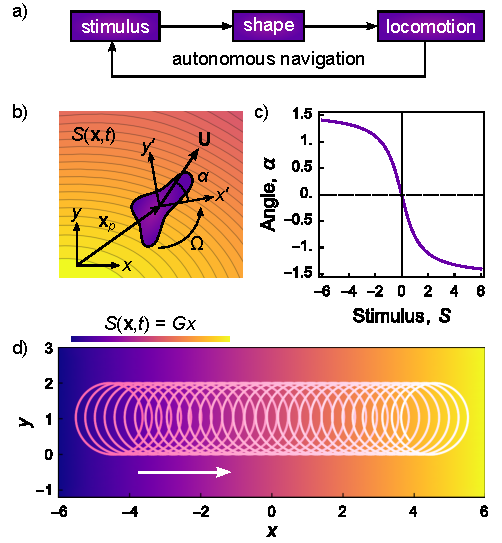
\includegraphics{figures/4_1.pdf}
     \caption{
     (a) A local stimulus determines particle shape which in turn directs particle motion towards new regions of the stimulus landscape.
     (b) An active particle moves with linear velocity $\ve{U}= U\cos\alpha \ve{e}_{x'} + U\sin\alpha \ve{e}_{y'}$ and angular velocity $\Omega\ve{e}_{z'}$ across a two-dimensional stimulus landscape $S(\ve{x},t)$.  
     (c) Assuming $R=U/\Omega=\text{constant}$, particle trajectories are determined by the stimulus-dependent orientation of the propulsion velocity $\alpha(S)$. Here, the function $\alpha(S)$ encodes for positive chemotaxis---that is, autonomous motion toward regions of higher stimulus. 
     (d) Computed trajectory of the particle in (c) on a uniform stimulus gradient $S(\ve{x})=G x$ of magnitude $G=0.1$. Here, lengths are scaled by the curvature radius $R$.}
     \label{fig:4.1}
 \end{figure}
%%%%%%%%%%%%%%%%%%%%%%%%%%%%%%


%%%%%%%%%%%%%%%%%%%%%%%%%%%%%%
\section{Self-phoretic Clusters}  
In practice, the design of the response functions $U(S)$, $\alpha(S)$, and $\Omega(S)$ requires one to consider the specific mechanism(s) of particle propulsion and its dependence on particle shape. Here, we consider the self-phoretic propulsion of hard sphere clusters, which have been studied previously in theory \autocite{soto2014self, varma2018clustering} and experiment \autocite{niu2018dynamics, schmidt2019light}. Each sphere $j$ in the cluster emits a constant flux $A_j$ of some chemical species, which sets up a concentration field $c(\ve{x})$ around the composite particle. At small P\'eclet number ($\text{Pe}=UL/D\ll1$), the species concentration is governed by the Laplace equation for steady-state diffusion, $\nabla^2c=0$, subject to the following boundary condition on the surface $\mathcal{S}_j$ of each sphere $j$
\begin{equation}
   -D\ve{n} \cdot \nabla c(\ve{x}) = A_j \quad \text{for} \quad \ve{x}\in \mathcal{S}_j
\end{equation}
where $D$ is the species diffusivity, and $\ve{n}$ is the unit normal directed out from the spheres.  Far from the particle, the species concentration approaches a constant value $c^{\infty}$, which can be set to zero without loss of generality. The resulting concentration field $c(\ve{x})$ depends on the shape of particle---that is, the configuration of its component spheres---but not its position and orientation within the stimulus landscape.

Concentration gradients tangent to the surface of each sphere drive interfacial phoretic flows with velocity 
\begin{equation}
    \ve{u}(\ve{x})=-\mu_j (\ve{\delta}-\ve{n}\ve{n}) \cdot \nabla c\quad \text{for} \quad \ve{x}\in \mathcal{S}_j
\end{equation}
where  $\mu_j$ is the mobility coefficient of sphere $j$.  At low Reynolds number ($\text{Re}=\rho UL/\eta$), the resulting velocity and pressure fields are governed by the Stokes equations, $-\nabla p + \eta \nabla^2 \ve{u}=0$ and $\nabla \cdot \ve{u}=0$, where $\eta$ is the fluid viscosity.  The linear velocity $\ve{U}$ and angular velocity $\ve{\Omega}$ of the rigid cluster is determined by the condition that there is no net force or torque on the particle.  We use a far-field approximation based on the method of reflections \autocite{varma2018clustering} to solve both the diffusion and hydrodynamic problems outlined above and estimate the particle velocity as a function of its shape \autocite{Supp}. For simplicity, we focus on the specific case of homogeneous clusters with $A_j=A$ and $\mu_j=\mu$; however, the model can also describe heterogeneous clusters made from spheres of different types.  We scale lengths by $L$, concentrations by $A L/D$, and velocities by $\mu A/D$, such that the velocities $\ve{U}$ and $\ve{\Omega}$ are determined entirely by particle geometry. \resp{Fig.\ \ref{fig:4.2}a shows the circular motion of an asymmetric three-sphere cluster as prescribed by the specific values of the sphere radii $a_i$ and the sphere-sphere separations $L_i$.}  

\section{Shape-shifting Clusters}  
In addition to shape-directed particle motion, we must also consider the effects of shape-shifting whereby the particle shape changes in response to changes in the local stimulus $S(\ve{x}_p,t)$.  Such particles can now be realized in experiment using stimuli responsive soft materials such as shape-changing polymers \autocite{magdanz2014stimuli} or liquid crystal elastomers \autocite{palagi2016structured} to alter the sizes and/or relative positions of spheres in the cluster.  In the present model, we consider a highly idealized form of shape-shifting, in which the bond lengths between neighboring spheres can depend on the local stimulus.  Fig.\ \ref{fig:4.2}b shows one example of a three-sphere cluster containing one stimuli-responsive bond.

%%%%%%%%%%%%%%%%%%%%%%%%%%%%%%
%%%%%%%%%%%%%%%%%%%%%%%%%%%%%%
\begin{figure}[!h]
    \centering
    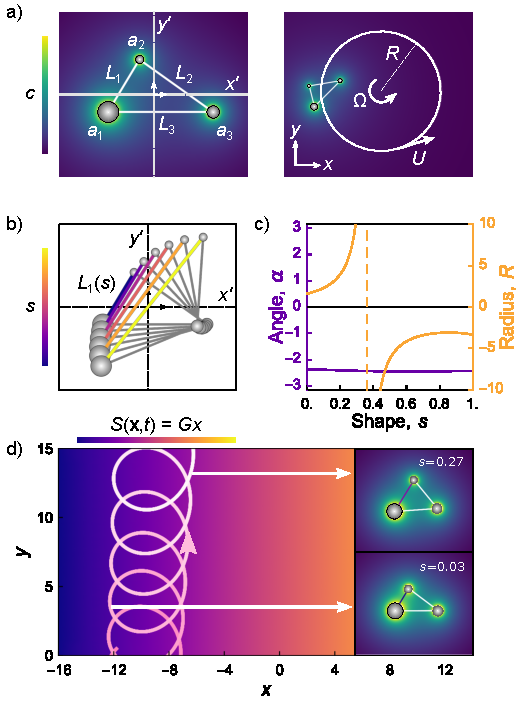
\includegraphics[width=8.5cm]{figures/4_2.pdf}
    \caption{Shape-shifting self-phoretic clusters. (a) Spheres connected by rigid bonds emit a chemical species that drives phoretic flows and particle motion with linear velocity $\ve{U}$ and angular velocity $\Omega$. Rigid particles move along circular trajectories of (signed) radius $R=U/\Omega$ (right). 
    (b) Standard shapes for different values of the shape parameter $s=(L_1-L_{\min})/(L_{\max}-L_{\min})$, which controls the length of one bond. The sphere positions $\ve{x}'_j(s)$ in the particle frame are chosen to eliminate particle translation and rotation due to shape change. 
    (c) Response functions $R(s)=U(s)/\Omega(s)$ and $\alpha(s)$ for the standard shapes in (b). 
    (d) Computed particle trajectory on a uniform stimulus gradient $S(\ve{x})=Gx$ of magnitude $G=0.2$; the shape parameter is assume to vary with the local stimulus as $s = (1+ e^{-S})^{-1}$. 
    In (a-d), the sphere radii are $a_1=0.1$, $a_2=0.04$, $a_3=0.06$; the fixed bond lengths are $L_2=0.860$ and $L_3=1$; the length of the responsive bond $L_1$ varies from $L_{\min}=0.5$ to $L_{\max}=1.5$.}
     \label{fig:4.2}
 \end{figure}
%%%%%%%%%%%%%%%%%%%%%%%%%%%%%%

To describe the motion of shape-shifting particles, we define a set of standard shapes that specify the position $\ve{x}_j'(s)$ of each sphere in the particle frame as a function of the shape parameter $s$ \autocite{shapere1989geometry}.  The standard shapes are chosen such that the particle frame does not translate or rotate within the viscous fluid as the particle changes its shape \autocite{Supp}.  In this way, we effectively remove the effects of particle swimming due to shape change, allowing us to focus exclusively on shape-induced changes in the propulsion velocity.  

For each standard shape, we compute the linear velocity $\ve{U}$ and angular velocity $\ve{\Omega}$ of the cluster as described above to obtain the response functions $U(s)$, $\alpha(s)$, and $\Omega(s)$. Fig.\ \ref{fig:4.2}c shows the response functions for a triangular cluster as a function of its one stimuli-responsive bond length, $s = (L_1 - L_{\min})/(L_{\max}-L_{\min})$.  This particle exhibits drifting motions in a stimulus gradient, but not the desired chemotactic motions parallel to the gradient direction (\resp{Fig.\ \ref{fig:4.2}d}).  In general, clusters will not satisfy the design criterion for chemotaxis that $R=\text{constant}$; however, it is possible to optimize their response by modifying the particle geometry.

\section{Design of Chemotactic Clusters} In designing chemotactic clusters that navigate up (or down) stimulus gradients, we seek to alter the cluster geometry such that each of the standard shapes leads to self-phoretic motion with a constant (signed) radius $R_0$. The design process can be formulated as an optimization problem that seeks to minimize the objective
\begin{equation}
    O(\ve{d}) = \langle [R(s,\ve{d})-R_0]^2 \rangle_s
\end{equation}
Here, the cluster geometry is parameterized by both the shape parameter $s\in[0,1]$ and the design variable $\ve{d}$, which is held fixed during shape-shifting.  The angle brackets denote averages over the shape parameter $s$, and $R(s,\ve{d})$ is the computed radius of the particle trajectory.

For the three-sphere cluster in Fig.\ \ref{fig:4.2}a, the design variable $\ve{d}$ includes two of the three radii ($a_2,a_3$) and one of the three bond lengths ($L_2$). All lengths are scaled by the length of the third bond $L_3$ such that $L_3\rightarrow 1$; the sphere radius $a_1$ is specified such that $a_1\ll L$ \resp{as required by the approximate model of phoretic propulsion outlined above}. The length $L_1$ of the stimulus-responsive bond is constrained to vary between user-specified limits $L_{\min}$ and $L_{\max}$. For each design $\ve{d}$, we compute the radius $R(s,\ve{d})$ of the particle trajectory as a function of the shape parameter using the model.  Numerical optimization methods can then be applied to identify the optimal shape-shifting particle.

Fig.\ \ref{fig:4.3}a highlights the performance of three different optimization methods based on hill climbing, random search, and the covariance matrix adaptation evolution strategy (CMA-ES) \autocite{hansen2016cma}, as applied to the design of chemotactic three-sphere clusters.  Greedy search algorithms such as hill climbing are quickly trapped in local minima; random searches are more effective but fail to identify the deepest minima.  The CMA-ES algorithm, which has proven effective on other problems involving colloidal clusters \autocite{miskin2013adapting}, combines stochastic ``mutation'' events with a deterministic ``selection'' process to identify optimal cluster geometries.  Fig.\ \ref{fig:4.3}b shows the optimal design for a three-sphere cluster with one stimuli-responsive bond.  Variations in the radius $R$ are ca.\ 2\% of the prescribed value (Fig.\ \ref{fig:4.3}c).  The orientation of the propulsion velocity $\alpha(s)$ decreases almost linearly with the shape parameter $s$ over a range spanning ca.\ 60$^{\circ}$. Assuming a sigmoidal response of the shape parameter on the local stimulus, the designed particle moves steadily up an applied stimulus gradient (positive chemotaxis; Fig.\ \ref{fig:4.3}d).

%%%%%%%%%%%%%%%%%%%%%%%%%%%%%%
\begin{figure}[!h]
    \centering
    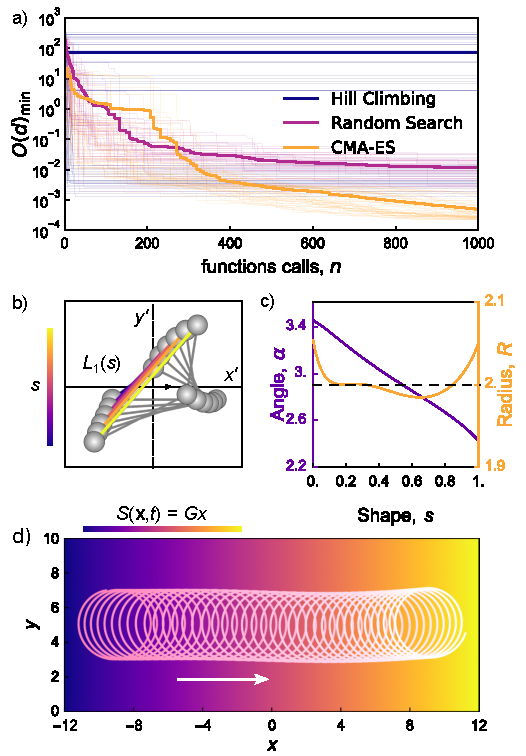
\includegraphics[width=8.5cm]{figures/4_3.pdf}
    \caption{Design of a chemotactic three-sphere cluster. (a) Minimum objective function $O(\ve{d})$ identified after $n$ function evaluations for three optimization methods initialized from 50 randomly selected designs (light curves); bold curves show the average performance. (b) Standard shapes for the optimal design for different values of the shape parameter $s=(L_1-L_{\min})/(L_{\max}-L_{\min})\in [0,1]$. During optimization, we prescribe the lengths $L_3=1$, $L_{\min}=0.5$, $L_{\max}=1.5$, $a_1=0.1$, and $R_0=2$; the optimal design identified is $a_2=0.0985$, $a_3=0.0958$, and $L_2=0.677$. (c) Computed response functions $\alpha(s)$ and $R(s)=U(s)/\Omega(s)$ for the standard shapes in (b). (d) Computed particle trajectory on a uniform stimulus gradient $S(\ve{x})=Gx$ of magnitude $G=0.2$; the shape parameter is assume to vary with the local stimulus as $s = (1+ e^{-S})^{-1}$.}
    \label{fig:4.3}
\end{figure}
%%%%%%%%%%%%%%%%%%%%%%%%%%%%%%

For spheres with the same activity and mobility connected by the same type of stimuli responsive bonds, one can design other particle clusters that behave in the opposite manner and swim down an applied gradient \autocite{Supp}.  Moreover, by altering the objective function, one can design particle clusters that navigate perpendicular to the gradient in a specified direction \autocite{Supp}. In addition to shape-shifting bonds between rigid spheres, one can also use responsive spheres that swell or shrink in response to local conditions. More generally, the present navigation strategy can be applied whenever particle motion depends on the local stimulus magnitude. Particle shape provides one of several possible design strategies for mediating this relationship between stimulus and motion.

\section{Effects of Noise} 
The type of autonomous navigation described here is only effective when rotational diffusion is slower than self-phoretic particle rotation.  Accounting for the particle's Brownian motion, the drift velocity in a uniform stimulus gradient $S(\ve{x},t)=G x$ can be approximated as $\ve{V}=-\tfrac{1}{2} G U R \alpha' \text{Pe}^2_r / (1+ \text{Pe}_r^2) \ve{e}_x +\mathcal{O}(G^2)$, where $\text{Pe}_r =\Omega\xi_r/k_B T$ is a rotational P\'eclet number, $\xi_r$ is a rotational friction coefficient (e.g., $\xi_r=8\pi\eta a^3$ for a sphere in an unbounded fluid), and $k_B T$ is the thermal energy.  As detailed in \autocite{Supp}, the derivation of this expression assumes that both the linear and angular propulsion velocity are independent of the stimulus (i.e., $U(S)=U$ and $\Omega(S)=\Omega$) and that the angular response function $\alpha(S)$ is approximately linear over changes in stimulus of order $GR$.  

For large P\'eclet numbers ($\text{Pe}_r\gg1$), the particle maintains orientational correlations over the duration of each circular orbit and uses this information to guide its motion on the stimulus landscape.  By contrast, rotational diffusion at small P\'eclet numbers ($\text{Pe}_r\ll1$) acts to erase these correlations thereby prohibiting effective navigation. Approximating the particle as a thin disk of diameter $L$ (such that $\xi_r=\tfrac{4}{3}\eta L^3$ \autocite{Kim2005}), the minimum particle size required for effective navigation ($\text{Pe}_r\sim1$) is $L\sim(3k_B T/4\Omega\eta)^{1/3}$.  Assuming a typical phoretic velocity of $\Omega=1$ rad/s, autonomous navigation in water ($\eta=10^{-3}$ Pa s) at room temperature requires particles sizes of order $L\sim 1~\mu$m or larger. Perhaps not surprisingly, this length is comparable to that of chemotactic bacteria such as \emph{E. coli}. \resp{Fig.\ \ref{fig:4.4} shows the  simulated  particle  motions  on  non-uniform gradients in the presence of Brownian motion.}

%%%%%%%%%%%%%%%%%%%%%%%%%%%%%%
\begin{figure}[h!]
     \centering
     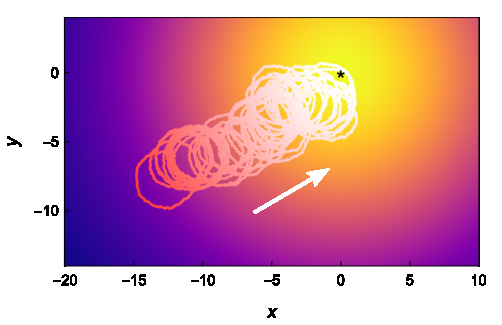
\includegraphics[width=8cm]{figures/4_4.pdf}
     \caption{\resp{Computed trajectory of the shape-shifting particle in Fig. \ref{fig:4.3}b-d moving on a peaked stimulus landscape with thermal noise. The stimulus is a Gaussian peak of width $\sigma=10$ and gradient magnitude $G=0.2$ centered at the origin, $S(x,y)= \sigma G  e^{-(x^2+y^2)/2\sigma^2}$; the  P\'eclet number is $Pe_r = 1000$.}}
     \label{fig:4.4}
 \end{figure}
%%%%%%%%%%%%%%%%%%%%%%%%%%%%%%

\section{Conclusions}  In sum, the shape-directed dynamics of shape-shifting particles provides a viable strategy for designing active colloids capable of autonomous navigation through heterogeneous environments.  While the present model focuses on self-phoretic motion, similar strategies should apply to other propulsion mechanisms that depend on particle shape (e.g., those based on external electric \autocite{Ma2015} or magnetic \autocite{Driscoll2017} fields).  The design of desired responses requires predictive understanding of both the relationship between stimulus and shape as well as the relationship  between shape and motion.  This design problem is simplest when the processes of shape-shifting and of shape-directed motion are effectively decoupled (e.g., when the former is much faster than the latter as assumed here). 

Recent advances in combining active colloids and stimuli-responsive materials should provide a promising platform to apply the design principles outlined here \autocite{Alvarez2019}. \resp{One significant challenge, however, is the often slow response times of existing shape-changing materials, which may be slower than that of particle propulsion (e.g., $\Omega^{-1}\sim 1$ s for phoretic propulsion). Experimental efforts to realize the proposed navigation strategy should therefore focus on shape-changing materials with fast response times such as some liquid crystal elastomers (LCEs) \autocite{camacho2004fast}.  Material deformations based on stimuli-dependent phase transitions should enable particles to navigate even small stimulus variations $\delta S$ about the transition $S_l$ where $\delta S \sim S_s \ll S_l$.  By incorporating material sensors and actuators, shape-shifting clusters can navigate autonomously on stimulus landscapes without the use of gradient-driven torques to bias their motion.} Looking forward, autonomous navigation based on internal degrees of freedom could be combined with external control strategies \autocite{liebchen2019optimal} to create colloidal robots capable of increasingly intelligent functional behaviors.

%\paragraph{\ydnote{Experimental realization guide }}
%\ydnote{Here we provide some basic guides to experimentally realize our proposed  shape-shifting autonomous navigation models. First, the choices of self-propulsion mechanism are not limited to the autophoretic particles. Any actuation mechanism(such as induced charge electrophoresis\autocite{brooks2018shape}, light induced thermophoresis\autocite{lozano2016phototaxis}, acoustic actuation\autocite{sabrina2018shape},  catalytic  self-electrophoresis\autocite{brooks2019shape})  for active colloids can be considered based on the materials of particles. Second,the candidates for shape-shifting materials including shape memory polymers/hydrogel \autocite{kirillova2019shape}, shape memory alloys \autocite{rodrigue2017overview}, liquid crystal elastomer\autocite{palagi2016structured} or composite materials\autocite{hu2018small}, etc. Shape-shifting materials can be the joints between active particles or active particles themselves.  The microstuctured particles can be farbricated with MEMS tech or chemical synthesis\autocite{leong2009tetherless}. One thing need to emphasized here that actuation source should be different from the shape-shifting source. For example, the particles can be light responsive shape-shifting driven by induced charge electrophoresis. Third, a physics model such as the autophoretic clusters model in this paper should be built to express relations between particles' shape and velocity.In the partical experiment model, an relaxation time $\tau_{relaxation}$ can be added to represent the reponse speed of the material to the stimulus. Shape of particles and shape-shifting path then can be designed following this paper's strategy to achieve the desired autonomous navigation behaviors.}






%%%%%%%%%%%%%%%%
% Chapter 5
%%%%%%%%%%%%%%%%
\chapter{Autonomous navigation of micro-magnetic rollers} \footnotetext{This chapter is adapted from Dou, Yong, and Kyle JM Bishop. "Autonomous navigation of shape-shifting microswimmers." Physical Review Research 1.3 (2019): 032030.}
\section{Introduction}
\section{Experiment}
\section{Discussion}
\section{Conclusion}

%%%%%%%%%%%%%%%%
% Conclusion
%%%%%%%%%%%%%%%%



\begin{center}
\pagebreak
\vspace*{5\baselineskip}
\textbf{\large Conclusion }
\end{center}


\begin{flushleft}
\hspace{10mm}Use this page for your epilogue or conclusion if applicable; please use only one of the titles for this page. Otherwise, you may delete it.
\end{flushleft}


%\pagenumbering{gobble}  %remove page number on summary page



\addcontentsline{toc}{chapter}{Conclusion and Outlook}


%%%%%%%%%%%%%%%%
% References
%%%%%%%%%%%%%%%%

\titleformat{\chapter}[display]
{\normalfont\bfseries\filcenter}{}{0pt}{\large\bfseries\filcenter{#1}}  % Reset title format for Reference section. (It is different from Chapter titles)
\titlespacing*{\chapter}
  {0pt}{0pt}{30pt}




\begin{singlespace}  % use single-line spacing for multi-line text within a single reference
	\setlength\bibitemsep{\baselineskip}  %manually set separataion betwen items in bibliography to double space
	\printbibliography[title={References}]
\end{singlespace}









\addcontentsline{toc}{chapter}{References}  %add References section to Table of Contents

%%%%%%%%%%%%%%%%
% Appendices
%%%%%%%%%%%%%%%%

%Readjust Title format for Appendicies
\titleformat{\chapter}[display]
{\normalfont\bfseries\filcenter}{}{0pt}{\large\chaptertitlename\ \large\thechapter : \large\bfseries\filcenter{#1}}  
\titlespacing*{\chapter}
  {0pt}{0pt}{30pt}	%controls vertical margins on title
  
% Adjust section title formatting
\titleformat{\section}{\normalfont\bfseries}{\thesection}{1em}{#1}

% Adjust subsection title formatting
\titleformat{\subsection}{\normalfont}{\thesubsection}{0em}{\hspace{1em}#1}

\begin{appendices}

%Some Table of Contents entry formatting
\addtocontents{toc}{\protect\renewcommand{\protect\cftchappresnum}{\appendixname\space}}
\addtocontents{toc}{\protect\renewcommand{\protect\cftchapnumwidth}{6em}}

%Begin individual appendices, separated as chapters

\chapter{ Experimental Equipment}
Lorem ipsum dolor sit amet, consectetur adipiscing elit, sed do eiusmod tempor incididunt ut labore et dolore magna aliqua. Ut enim ad minim veniam, quis nostrud exercitation ullamco laboris nisi ut aliquip ex ea commodo consequat. Duis aute irure dolor in reprehenderit in voluptate velit esse cillum dolore eu fugiat nulla pariatur. Excepteur sint occaecat cupidatat non proident, sunt in culpa qui officia deserunt mollit anim id est laborum.

\chapter{Data Processing}
Lorem ipsum dolor sit amet, consectetur adipiscing elit, sed do eiusmod tempor incididunt ut labore et dolore magna aliqua. Ut enim ad minim veniam, quis nostrud exercitation ullamco laboris nisi ut aliquip ex ea commodo consequat. Duis aute irure dolor in reprehenderit in voluptate velit esse cillum dolore eu fugiat nulla pariatur. Excepteur sint occaecat cupidatat non proident, sunt in culpa qui officia deserunt mollit anim id est laborum.

\end{appendices}

\end{document} 
